% 
% Dissertação de Mestrado
% Mestrado IC-UNICAMP
% Novembro 2009
% Autor: Thiago Alvarenga Lechuga (thiagoalz@gmail.com)
% IC-UNICAMP
% http://www.ic.unicamp.br/~079699
%

%USADOS COMO BASE: Qualificação, Artigo SAC, Artigo WBPM

%\documentclass[12pt,twoside]{report} % Use esta linha para tese com mais de 100 p{\'a}ginas
\documentclass[12pt]{report} % Use esta linha para tese com at{\'e} 100 p{\'a}ginas

% *** GRAPHICS RELATED PACKAGES ***
\usepackage[pdftex]{graphicx}
%declare the path(s) where your graphic files are
\graphicspath{{imagens/}{images/}}
%and their extensions so you won't have to specify these with
%every instance of \includegraphics
\DeclareGraphicsExtensions{.pdf,.jpeg,.png}


\usepackage{ic-tese}
\usepackage[utf8]{inputenc}
%\usepackage[latin1]{inputenc}
\usepackage[brazil]{babel}

%para ordenar as citações direitinho automaticamente
\usepackage[sort]{cite}

%Para quebrar e linkcar as urls corretamente
\usepackage{url}
\newcommand{\acesso}{. Acessado em março de 2010}

%para criar o indice e links no PDF
\usepackage{hyperref}

%para adicionar codigo
\usepackage{listings}

%poder criar tabelas com multirow
\usepackage{multirow}

%Adicionar pdf(artigo) nos apendices
\usepackage{pdfpages}

%CONFIGURANDO AUTOREF
\def\figureautorefname{Figura}
\def\tableautorefname{Tabela}
\def\appendixautorefname{Apêndice}
\def\chapterautorefname{Capítulo}
\def\sectionautorefname{Sessão}
\def\subsectionautorefname{Sessão}
\def\subsubsectionautorefname{Sessão}
\def\equationautorefname{Fórmula}
%\def\lstlistingautorefname{Alg.}
%%%%%%%%%%%%%%%%%%%

%%%%%%%%%%%Setando variáveis%%%%%%%%%%%%%%%%%%%%%%%%%%
%%Mudei de lugar para poder usar as variáveis nas configurações do hyperref
% \title{Como Escrever um T{\'\i}tulo em Duas Linhas\\
% 	para sua Disserta\c{c}{\~a}o ou Tese}
\title{Uma Proposta de Meta-Escalonamento e Execução de Workflows WS-BPEL em Ambientes Multi-Cluster}
\author{Thiago A. Lechuga}
\degreesought{Mestrado} % Doutorado/Mestrado
\titlesought{Mestre}     % Doutor/Doutora/Mestre
\principaladvisor{Profª. Drª. Maria Beatriz Felgar de Toledo}
\advisortitle{Orientadora} % Orientador/Orientadora
%\coadvisor{Byron Meter (Co-orientador)} % Pode ser omitido.
\firstreader{Prof. Dr. Mario Antonio Ribeiro Dantas\\ Centro Tecnológico / UFSC}
\secondreader{Prof. Dr. Edmundo Roberto Mauro Madeira\\ IC / UNICAMP}
\thirdreader{Profª. Drª. Islene Calciolari Garcia (Suplente)\\ IC / UNICAMP}
\fourthreader{Prof. Dr. Eleri Cardozo (Suplente)\\ FEEC / UNICAMP}
\grants{{\rm Suporte financeiro de: Bolsa CNPq (processo 135020/2008-5) 2008--2009, Bolsa FAPESP (processo 2008/52867-0)
2009--2010.}} % Pode ser omitido.
%
\submitdate{Outubro de 2010} % Pode ser omitido.
\date{21 de outubro de 2010} % Pode ser omitido.
%%%%%%%%%%%%%%%%%%%%%%%%%%%%%%%%%%%%%%%%%%%%%%%%%%%%%%%

%%Para permitir o uso das variaveis \@author e \@title
\makeatletter
\AtBeginDocument{\markboth{\@author}{\@title}} 

%%%%%%% Configurando o hyperref
\hypersetup{
    %bookmarks=true,         % show bookmarks bar?
    unicode=false,          % non-Latin characters in Acrobat’s bookmarks
    pdftoolbar=true,        % show Acrobat’s toolbar?
    pdfmenubar=true,        % show Acrobat’s menu?
    pdffitwindow=false,     % window fit to page when opened
    pdfstartview={FitH},    % fits the width of the page to the window
    pdftitle={\@title},    % title
    pdfauthor={\@author},     % author
    pdfsubject={Dissertação de Mestrado},   % subject of the document
    pdfcreator={\@author},   % creator of the document
    pdfproducer={UNICAMP}, % producer of the document
    pdfkeywords={BPEL; Cluster of Clusters; Workflow}, % list of keywords
    pdfnewwindow=true,      % links in new window
    colorlinks=true,       % false: boxed links; true: colored links
    linkcolor=black,          % color of internal links
    citecolor=black,        % color of links to bibliography
    filecolor=black,      % color of file links
    urlcolor=black,           % color of external links
    %linkbordercolor={1 1 1},
    %citebordercolor={1 1 1},
    breaklinks=true,
}

%%%%%%%%%%%%%%%%%%%%%%%%%%%%%%%
%configurações para códigos inseridos
\lstset{
    language=XML,                   % choose the language of the code
    basicstyle=\footnotesize,       % the size of the fonts that are used for the code
    numbers=left,                   % where to put the line-numbers
    numberstyle=\footnotesize,      % the size of the fonts that are used for the line-numbers
    stepnumber=1,                   % the step between two line-numbers. If it's 1 each line will be numbered
    numbersep=10pt,                 % how far the line-numbers are from the code
    backgroundcolor=\color{white},  % choose the background color. You must add \usepackage{color}
    showspaces=false,               % show spaces adding particular underscores
    showstringspaces=false,         % underline spaces within strings
    showtabs=false,                 % show tabs within strings adding particular underscores
    frame=single,                   % adds a frame around the code
    tabsize=2,                      % sets default tabsize to 2 spaces
    captionpos=b,                   % sets the caption-position to bottom
    breaklines=true,                % sets automatic line breaking
    breakatwhitespace=false,        % sets if automatic breaks should only happen at whitespace
    escapeinside={\%*}{*)}         % if you want to add a comment within your code
%     extendedchars=\true,
%     inputencoding=utf8   
    }
    %Passei esses comandos pro sty.
    %\renewcommand\lstlistingname{Código}
    %\renewcommand*{\lstlistlistingname}{Lista de Listagens}


%%%%%%%%%%%%%%%%%%%%%%%%%%%%%%%%
%Para tirar a hyphenation e justificar :D
%%%%%%%%%
% \tolerance=1
% \emergencystretch=\maxdimen
% \hyphenpenalty=10000
% \hbadness=10000
%%%%%%%%%

% %TODO: Tabela de siglas?

\begin{document}
%
%   Se pretende utilizar \copyrighttrue, consulte antes seu orientador ou a CPG!!!
%   Este ponto envolve quest{\~o}es legais complexas e de graves conseq{\"u}{\^e}ncias.
\copyrightfalse % Caso nao queira que apareca a pagina de Copyright.
%    \copyrighttrue % Caso queira que apareca a pagina de Copyright.
%
\finalversiontrue % Caso seja a versao final.
%\finalversionfalse % Caso nao seja a versao final ainda.
%
\tablespagetrue % Caso queira que apareca a Lista de Tabelas.
%\tablespagefalse % Caso nao queira que apareca a Lista de Tabelas.
%
\figurespagetrue % Caso queira que apareca o Lista de Figuras.
%\figurespagefalse % Caso nao queira que apareca o Lista de Figuras.

\listingspagetrue % Caso queira que apareca o Lista de Listagens. O pacote Listings deve estar sendo usado (\usepackage{listings})
%\listingspagefalse % Caso nao queira que apareca o Lista de Listagens.
%
\beforepreface


%%%%%% Epígrafe %%%%%%%%
\prefacesection{}
  \vfill
  \begin{flushright}    
    \textit{Knowledge is only useful if you can share it.}\\
    Autor desconhecido.
  \end{flushright}

\prefacesection{Resumo}
    
    A utilização de sistemas distribuídos heterogêneos, tais como os \textit{Multi-Clusters}, também chamados de \textit{Clusters} de \textit{Clusters} (CoC), e as grades computacionais, permite o desenvolvimento de sistemas computacionais mais complexos.
    No entanto, alguns desses sistemas requerem que os serviços sejam facilmente compostos e executados, mantendo as dependências entre eles;
    ambos, serviços e dependências, podem ser representados como \textit{workflows}.
    Ainda, os serviços Web foram adotados na estrutura desses sistemas distribuídos, e WS-BPEL é o padrão para a sua composição.
    Portanto, o objetivo deste trabalho é permitir a execução de \textit{workflows} escritos em WS-BPEL em \textit{Multi-Clusters}.
    Para alcançar esse objetivo, uma extensão da linguagem WS-BPEL é apresentada incluindo a especificação de qualidade de serviço (QoS), juntamente com os recursos necessários para execução dos serviços no CoC.
    Além disso, este trabalho apresenta uma infraestrutura que permite a execução de \textit{workflows} em CoC, e um estudo de caso utilizando a SHARCNET, a fim de avaliar a abordagem proposta.
    Finalmente, um \textit{workflow} científico real para gerar mosaicos personalizados do céu é implementado usando o ambiente criado.      

\prefacesection{Abstract}    

    The use of heterogeneous distributed systems, such as Multi-Clusters, as known as Cluster of Clusters (CoC), and computational grids, enables the development of complex computational systems.
    However some of these systems require services to be easily composed and executed while maintaining the dependencies among them;
    both the services and the dependencies can be represented as workflows.
    Moreover, Web Services have been adopted in distributed systems, and WS-BPEL is the standard for Web Services composition.
    Accordingly, the objective of this work is to enable the execution of WS-BPEL workflows in a CoC.
    In order to achieve this execution, an extension to the WS-BPEL language is presented that includes the specification of Quality of Services (QoS), along with the required computational resources for service execution in CoCs.
    Additionally, this paper presents an infrastructure that enables the execution of such workflows in CoCs, and a case study using SHARCNET is discussed in order to evaluate the proposed approach.
    Finally, a real scientific workflow to generate custom mosaics of the sky is implemented using the criated environment.    
   

\prefacesection{Agradecimentos}
    Apesar de o título que esta dissertação busca ser individual, de forma alguma a trajetória para chegar até aqui seria cumprida dessa forma.
    Gostaria, portanto, de dedicar essas linhas a agradecer a pelo menos uma parte das pessoas que tornaram mais esse objetivo possível.
    
    Primeiramente à \textbf{Deus}, à \textbf{Vida} e ao meus pais, \textbf{Willian} e \textbf{Lourdes}, que me educaram e apoiaram, sendo assim os responsáveis por tudo o que sou hoje.
    Amo vocês.%TODO:Melhorar
    
    À toda a minha família, à minha vó, \textbf{Maria}, e aos meus tios e tias, \textbf{Esther}, \textbf{Elísio}, \textbf{Imaculada}, \textbf{Carlos}, \textbf{Geraldo}, \textbf{Lúcia}, \textbf{Yvonne} e \textbf{Magno}. 
    De ajudando na mudança a diminuindo minha pilha de roupas sujas, cada um emprestou um pouco de si para me apoiar nessa jornada.
    Eu poderia passar horas escrevendo as inúmeras maneiras que vocês me ajudaram, mas nada disso se compara a companhia, carinho, amor e afeto que recebi como se eu ainda fosse o pequeno sobrinho/neto que se mudou para longe a mais de 10 anos. Amo todos vocês.
    Não poderia esquecer de mandar um abraço especial para meus irmãos, primos e primas e para meu avô, \textbf{Edgard}, que, esteja onde estiver, sei que cuida muito bem de todos nós e está muito contente com essa conquista.    

    À \textbf{Camila} e meus grandes amigos, \textbf{Diogo}, \textbf{Henrique} e \textbf{Leonardo}, que hoje já me apoiaram em uma grande parcela da minha vida.
    Perto ou longe, algumas pessoas são para a vida toda.

    À minha orientadora, Prof. \textbf{Maria Beatriz}. Obrigado pelo tempo, orientação e paciência.

    A todas as pessoas que me receberam e me ajudaram no Canadá.
    À Prof. \textbf{Miriam}, ao \textbf{Américo}, ao \textbf{Mário} e ao \textbf{Lúcio}, obrigado pela orientação, ajuda, apoio e companhia de todos.
    Aos grandes novos amigos que tornaram minha estadia nesse país gelado muito mais divertida e prazerosa, \textbf{Elisa}, \textbf{Fabrício}, \textbf{Lorena} e \textbf{Márcia}.
    Obrigado a todos, esse período estará para sempre gravado em minha memória com muita saudade.

    Aos amigos da UNICAMP e do mestrado, entre eles, \textbf{Cristiano}, \textbf{Daniel}, \textbf{Douglas}, \textbf{Faveri}, \textbf{Guilherme}, \textbf{Isaura}, \textbf{Marcos}, \textbf{Maria}, \textbf{Robinho}, \textbf{Tripodi}, \textbf{Willian}.
    Obrigado pela companhia, pelos dias divertidos, pelas risadas e por toda a \emph{fundamental} ajuda.
    Sem vocês eu ainda estaria procurando tempo para estudar grafos.
    Podem ter certeza que a minha gratidão é muito maior do que eu conseguiria expressar mesmo com a ``Perícia de cirurgião atômico da Noruega''. ;)
    Vou sentir muita falta de vocês.

    A todo o pessoal do laboratório e ao chefe \textbf{Tizzei}, que aguentaram pacientemente minhas bagunças e ainda estavam sempre dispostos a me ajudar com valiosas dicas.

    Por ultimo, e não menos importante, todas as outras pessoas que colaboram direta ou indiretamente e que, por falta de memória e/ou espaço, não estão nomeadas aqui. Um sincero OBRIGADO.

\afterpreface % Gera: Conteudo, Lista de Tabelas, Lista de Figuras.
%

\chapter{Introdução}        
       
    %introducao
    Os \textit{clusters} de alta performance (HPCCs)~\footnote{Do inglês, \textit{High Performance Computing Clusters}} continuam sendo uma solução para a demanda computacional constantemente crescente de diversos institutos comerciais e de pesquisa.
    Entretanto, enquanto um \textit{cluster} é projetado para atender os picos de carga de uma organização, essa situação não ocorre com frequência, deixando o equipamento a maior parte do tempo ocioso.
    Portando, para otimizar a utilização dos seus recursos, diversas organizações tentem a compartilhar HPCCs.
    Assim, enquanto uma organização não utiliza seus recursos, outros parceiros podem utilizá-los, aumentando a capacidade máxima de processamento de ambas.   
    Então, ao invés de pequenos grupos de usuários tendo acesso exclusivo a um sistema específico, temos grandes grupos compartilhando diversos \textit{clusters}.
    Essa abordagem colaborativa pode maximizar a utilização dos recursos, permitir a implementação de tarefas mais complexas e reduzir o tempo de espera~\cite{Bauer06}.
	
    %Colocar algo sobre WF? BPEL? Orquestração?
	
    %Sit problema
    O uso de sistemas heterogêneos distribuídos, como os \textit{Multi-Clusters}, ou \textit{Clusters} de \textit{Clusters}(CoC)~\footnote{Do inglês, \textit{Cluster of Clusters}}, e as grades computacionais, permitem o estudo de diversos problemas que eram computacionalmente inviáveis em outros ambientes.
    Entretanto, alguns desses problemas são complexos e precisam ser facilmente compostos e executados, mantendo as dependências entre si.
    Embora serviços e dependências possam ser representadas através de \textit{wokflows}, os padrões atuais para a composição de serviços em sistemas distribuídos heterogêneos ainda são inadequadas.
    Como os serviços Web~\cite{alonso2004} (WS)\footnote{Do inglês, \textit{Web Services}} foram adotados na infraestrutura desses sistemas e como o WS-BPEL~\cite{bpel:website}, \textit{Web Services Business Process Execution Language}, é o padrão para a sua composição, essa linguagem se torna uma forte candidata para a utilização nesse novo cenário.
    Contundo, ainda existem requisitos específicos que devem ser considerados, como por exemplo a seleção de recursos baseada em requisitos não-funcionais~\cite{FOX06}.

    \section{Objetivos}
	O objetivo deste trabalho é possibilitar a especificação e execução de \textit{wokflows} especificados na linguagem WS-BPEL que utilizam recursos de \textit{Multi-Clusters}.
	Especificamente, as contribuições esperadas incluem: 
	\begin{itemize}
	 \item Uma extensão à linguagem WS-BPEL que permita especificação e seleção de recursos baseada em requisitos de qualidade de serviço (QoS)\footnote{Do inglês, \textit{Quality of Services}} e de recursos computacionais requeridos para a execução de cada serviço;
	 \item Uma sugestão de arquitetura para permitir a execução de \textit{workflows} em CoCs.
	 \item Implementação da arquitetura proposta em um ambiente de produção.
	 \item Especificação e implementação de um problema real no ambiente criado.
	\end{itemize}		
	
	% %justificativa?
	% %justificativa (1 paragrafo)
	% %Through the development of a new layer capable of operating as a global scheduler to the clusters, the system resources will be allocated more effectively, hence reducing waiting time. 
	% %In addition, the global scheduler would enable the SHARCNET to be used for the execution of BPEL workflows.

	%Metodologia?

    \section{Estrutura da Dissertação}    
	Esta dissertação contém mais cinco capítulos estruturados como descrito a baixo:
	
	\begin{itemize}
	 \item 	\autoref{chap:fundamentos}: Apresenta os conceitos básicos necessários para o entendimento deste trabalho.
	 Dividido em três sessões, fala sobre os conceitos de \textit{clusters}, computação orientada a serviços e orquestração de serviços;
	 \item 	\autoref{chap:RelatedWork}: Relaciona e compara alguns trabalhos relacionados. Divide-se em duas sessões.
	 Na \autoref{sec:RelatedWF} são levantados os trabalhos com o foco na execução de \textit{workflows} em sistemas distribuídos heterogêneos.
	 Na \autoref{sec:RelatedEscalonador} algumas pesquisas sobre escalonamento global, ou Meta-Escalonamento, em \textit{Multi-Clusters} são apresentadas;
	 \item	\autoref{chap:Desenvolvimento}: Descreve com detalhes as principais contribuições desenvolvidas neste trabalho.
	 A \autoref{sec:extendedBPEL} explica as adaptações feitas na linguagem WS-BPEL para permitir que requisitos de QoS e recursos necessários para a execução das tarefas sejam expressos na composição, condição necessária para a execução em CoCs.
	 Na \autoref{sec:ArquiteturaProposta} é proposta uma arquitetura para a execução de \textit{workflows} descritos em WS-BPEL que utilizam recursos de um CoC, permitindo seleção de recursos baseada em requisitos funcionais e não-funcionais.
	 Finalmente, a \autoref{sec:EstudoDeCasoSHARCNET} demonstra uma aplicação dessa arquitetura utilizando a rede SHARCNET como \textit{Multi-Cluster}, e ilustra detalhes da implementação, como o \texttt{Escalonador Global} (\autoref{subsec:EscalonadorGlobal}), o \texttt{Broker} (\autoref{subsec:Broker}), o \texttt{Mediador} (\autoref{subsec:Mediador}), o \texttt{Monitor} (\autoref{subsec:Monitor}), e outros elementos da arquitetura;
	 \item 	\autoref{chap:Aplicacao}: Demonstra uma aplicação de um problema real implementada utilizando as contribuições apresentadas neste trabalho;
	 \item 	\autoref{chap:Conclusao}: Conclui a dissertação destacando as contribuições e listando trabalhos futuros.
	\end{itemize}    

\chapter{Fundamentos}
\label{chap:fundamentos}    
    Neste capítulo, de caráter conceitual, serão apresentados os fundamentos necessários para o entendimento desta dissertação.
    Inicialmente, serão abordados os conceitos de \textit{Cluster} e \textit{Multi-Clusters}.
    Em seguida, os fundamentos de computação orientada a serviços são abordados, falando sobre os mecanismos de descoberta, descrição e comunicação dos serviços Web.
    Para concluir, o texto aborda os conceitos de \textit{workflows} e WS-BPEL, e os relaciona com os \textit{Multi-Clusters}.

    \section{Clusters}
	Na tentativa de resolver problemas com a complexidade cada vez maior utilizando computadores, a tendência natural foi criar processadores cada vez mais rápidos.
	Gordon Moore previu em 1965~\cite{moore} um crescimento quase que exponencial para os circuitos integrados, o que pode também ser refletido, de certa forma, na capacidade de processamento dos mesmos.
	Entretanto, esse crescimento está atingindo os limites da própria física e decaindo cada vez mais.
	Assim, na tentativa de transpor essas barreiras, as indústrias de microprocessadores estão investindo em novas tecnologias.
	Uma possível solução é o uso dos \textit{clusters} computacionais, também conhecidos na literatura em português por agregados computacionais~\cite{marioLivro}.	
	
	O processamento de alto desempenho (PAD), conhecido em inglês por \textit{High Performance Computing} (HPC), foi baseado durante muito tempo em computadores paralelos específicos, tais como aqueles com arquiteturas massivamente paralelas (MPP)\footnote{Do inglês, \textit{Massively Parallel Processor}} e os de memória compartilhada (SMP)\footnote{Do inglês, \textit{Shared Memory Processors}}.
	Contudo, devido ao alto custo de máquinas dos tipos MPP e SMP, além da grande oferta de computadores pessoais existentes nas redes das instituições, políticas de agregar máquinas estão sendo cada vez mais utilizadas~\cite{marioLivro}.

	\subsection{Classificação}
	    Atualmente não existe uma taxonomia globalmente aceita para os ambientes de \textit{clusters}.
	    Dantas~\cite{marioLivro} classifica os agregados usando cinco tipos de métricas:

	    \begin{itemize}
		\item \textbf{Limite Geográfico:}  Pequena, média e grande;
		\item \textbf{Utilização dos Nós:} Dedicados e não dedicados;
		\item \textbf{Tipo de Hardware:} NOW, COW e CLUMPS;
		\item \textbf{Aplicações Alvo:}  Alto desempenho e alta disponibilidade;
		\item \textbf{Tipos de Nós:}  Homogêneo, Heterogêneo.
	    \end{itemize}

	    A seguir cada uma das métricas anteriormente listada é detalhada e exemplificada.
	
	    \subsubsection{Limite Geográfico}
		As configurações podem variar desde a simples agregação de computadores do tipo PC utilizando \textit{hubs} ou \textit{switches}, até o uso de dispositivos especiais de interligação, como \textit{Myrinet}, \textit{Quadrics} e \textit{Memory Channel}.
		Na maioria das organizações os \textit{clusters} tendem a surgir em salas específicas e laboratórios, ou seja, locais com certa limitação geográfica.
		A partir do conhecimento adquirido por uma determinada equipe, o \textit{cluster} tende a crescer para uma configuração departamental.
		Finalmente, obtendo sucesso, o sistema pode se expandir para um nível organizacional com o intuito de propagar os benefícios do uso do paradigma.

	    \subsubsection{Utilização dos Nós}
		Este aspecto pode ser considerado um dos mais importantes a ser observado na formação de um \textit{cluster}.
		É fundamental que seja estabelecido a participação dedicada ou não-dedicada dos nós que irão compor o agregado.
		Fatores como políticas de gerenciamento, segurança, disponibilidade, escalonamento e balanceamento de carga estão relacionados diretamente à forma de utilização dos nós.

	    \subsubsection{Tipo de Hardware}
		Os tipos de \textit{hardware} empregados vem sendo classificados de uma forma empírica como \textit{Nows}, \textit{Cows} e \textit{Clumps}.
		
		As \textit{Nows} (\textit{Network of Workstations}) são caracterizadas pelo uso de estações de trabalho distribuídas em uma rede local.
		Configurações classificadas como \textit{Cows} (\textit{Cluster of Workstations}) se diferenciam das \textit{Nows} pelo uso de máquinas homogêneas e dedicadas à execução de aplicações específicas.
		Os \textit{Clumps} (\textit{Cluster of SMPs}) são ambientes compostos de máquinas com arquitetura SMP, anteriormente citada.
	    
	    \subsubsection{Aplicações Alvo}
		Com relação à necessidade das aplicações os \textit{clusters} geralmente se dividem em dois alvos principais: alto desempenho e alta disponibilidade.
		Embora também seja possível observar aplicações com os dois tipos de requisitos.
		
		No primeiro grupo as aplicações necessitam de alto desempenho para sua execução.
		Assim, um \textit{cluster} com um grande número de processadores, memória e disco, é o ambiente ideal para esse tipo de aplicação.
		
		Já para o outro grupo, no qual as aplicações precisam de alta disponibilidade, o agregado se mostra eficiente permitindo que a aplicação seja distribuída garantindo que esta não seja interrompida.
	    
	    \subsubsection{Tipos de Nós}
	    Outro fator importante a ser observado na classificação dos \textit{clusters} se refere à similaridade de \textit{hardware} e \textit{software} dos nós que compõem o ambiente.
	    Podendo ser agrupados em nós homogêneos e heterogêneos.	    
    

	\subsection{Multi-Clusters}
	    %TODO: Tentar melhorar mais coisas e mais exemplos de CoC
	    %TODO: Figura de cluster fo cluster?
	    Os \textit{High Performance Computing Clusters (HPCC)} continuam sendo uma solução comum para satisfazer a sempre crescente demanda computacional de diversos institutos comerciais e de pesquisa.
	    Entretanto, um único \textit{cluster} é normalmente planejado para suportar cargas máximas de trabalho de uma organização, que geralmente não acontecem com frequência.
	    Para otimizar o uso dos recursos, diversas organizações tendem a compartilhar HPCCs entre si.
	    Dessa forma, ao invés de pequenos grupos de usuário com acesso exclusivo para um \textit{hardware} específico, temos grupos maiores que compartilham diversos \textit{clusters}.
	    Essa abordagem pode potencializar o uso dos recursos, permitindo a execução de tarefas maiores e diminuindo o tempo de espera~\cite{Bauer06}.

	    Entretanto, para atingir tal nível de compartilhamento alguns desafios devem ser superados;
	    entre eles, está o gerenciamento dos recursos desse tipo de arquitetura, comumente chamada de \textit{Cluster} de \textit{Clusters} (CoC)\footnote{Na literatura inlgesa, \textit{Cluster of Clusters}}, ou Multi-Clusters.
	    Por esse motivo o escalonamento de tarefas em plataformas heterogêneas tornou-se recentemente alvo de pesquisas~\cite{Rauuber07}.

	    Como exemplo desse tipo de estrutura pode-se citar a SHARCNET~\cite{sharcnet:website}, uma rede multi-institucional de \textit{clusters} de alto desempenho, espalhada por 16 instituições acadêmicas na província de Ontário, Canadá.
	    O sistema citado não possui um escalonador global, por esse motivo a seleção de onde cada tarefa deve ser executada é feita de forma manual, obrigando o usuário a verificar quais sistemas estão ativos, e impedindo que suas tarefas sejam executadas de forma automatizada, como em um \textit{workflow}.
      

    \section{Computação Orientada a Serviços}
	Computação Orientada a Serviços é um paradigma de modelagem que especifica a criação da infraestrutura de \textit{software} de um determinado negócio em forma de serviços.
	Serviços podem ser definidos como componentes de software auto-descritivos que apoiam a composição ágil de aplicações~\cite{Leymann02webservices}.
	
	Esse modelo pode ser aplicado como estratégia para a implantação de uma arquitetura orientada a serviços, denominada SOA\footnote{Do inglês, \textit{Service-Oriented Architecture}}~\cite{SOAPapa}.
	Como outros paradigmas de modelagem, a orientação a serviços fornece meios para desacoplar interesses e fomentar o reuso.
                                   
	\subsection{SOA e Serviços Web}
	    Um sistema distribuído é composto por um conjunto de elementos de \textit{hardware} e \textit{software} que se comunicam através da troca de mensagens~\cite{Coulouris}.
	    A comunicação entre máquina e homem é algo já bastante difundido com a proliferação da Web e das tecnologias correlatas como, por exemplo, a linguagem HTML.
	    No entanto a possibilidade de efetuar interações entre máquina-máquina, ou melhor, aplicação-aplicação vem ganhando um espaço considerável na área da computação.
	    Algumas tecnologias já implementam mecanismos que possibilitam a execução de procedimentos remotos como, por exemplo, Sun RPC~\cite{Coulouris} e Java RMI~\cite{BeginingJava}.
	    Essas tecnologias possibilitam que uma aplicação invoque uma outra remotamente passando parâmetros de processamento e recebendo uma resposta como resultado de tal procedimento.           

	    Durante muitos anos, aplicações que necessitavam de algum tipo de comunicação externa interagiram através de soluções \textit{ad hoc}, utilizando a infraestrutura básica da internet~\cite{IntroWS}.
	    No entanto tais tecnologias são, em muitos casos, dependentes de plataformas e linguagens de programação, fato que as torna mais fechadas.
	    
	    As arquiteturas orientadas a serviços fazem uso extensivo da tecnologia de serviços Web de maneira a definir uma estrutura distribuída, independente de plataforma e linguagem de programação.
	    Assim, os serviços Web emergiram como um \textit{framework} sistemático e extensível para possibilitar a interação entre aplicações.
	    Um serviço Web, portanto, é um sistema de software projetado, utilizando um conjunto de padrões abertos, para permitir a interoperabilidade entre sistemas~\cite{alonso2004}.
	    Dessa forma, uma determinada aplicação pode ser implementada na forma de um serviço e disponibilizada para ser invocada remotamente.            

	    Na tentativa de ilustrar a utilização dos serviços Web em uma situação real, podemos imaginar um site de vendas pela Internet, que necessita validar o crédito do comprador antes de proceder com a venda.
	    O sistema então acessa um serviço (WS) que cuida de todos os passos necessários à verificação de crédito: verifica o histórico das compras efetuadas pelo consumidor na empresa, a situação de crédito do consumidor no sistema público, etc.
	    O serviço Web obtém estes dados e retorna a situação de crédito deste consumidor para o site.

	    %TODO:Definir o que é serviço Web e como é identificado (URI). Mais dados técnicos?
	    %Fazer o link com SOA.
		    
	    A estrutura SOA possui três camadas básicas: descoberta de serviços, descrição de serviços e protocolo de comunicação.
	    A \autoref{fig:SOA} mostra os protocolos mais comuns, e aceitos como padrão, para cada uma das três camadas; UDDI, WSDL e SOAP, respectivamente.
	    Cada uma delas será detalhada posteriormente.

	    A \autoref{fig:WS} ilustra, de uma maneira abstrata, o modelo empregado através da estrutura de camadas de serviços Web.
	    
	    \begin{figure}[!htb]
	    \begin{center}
		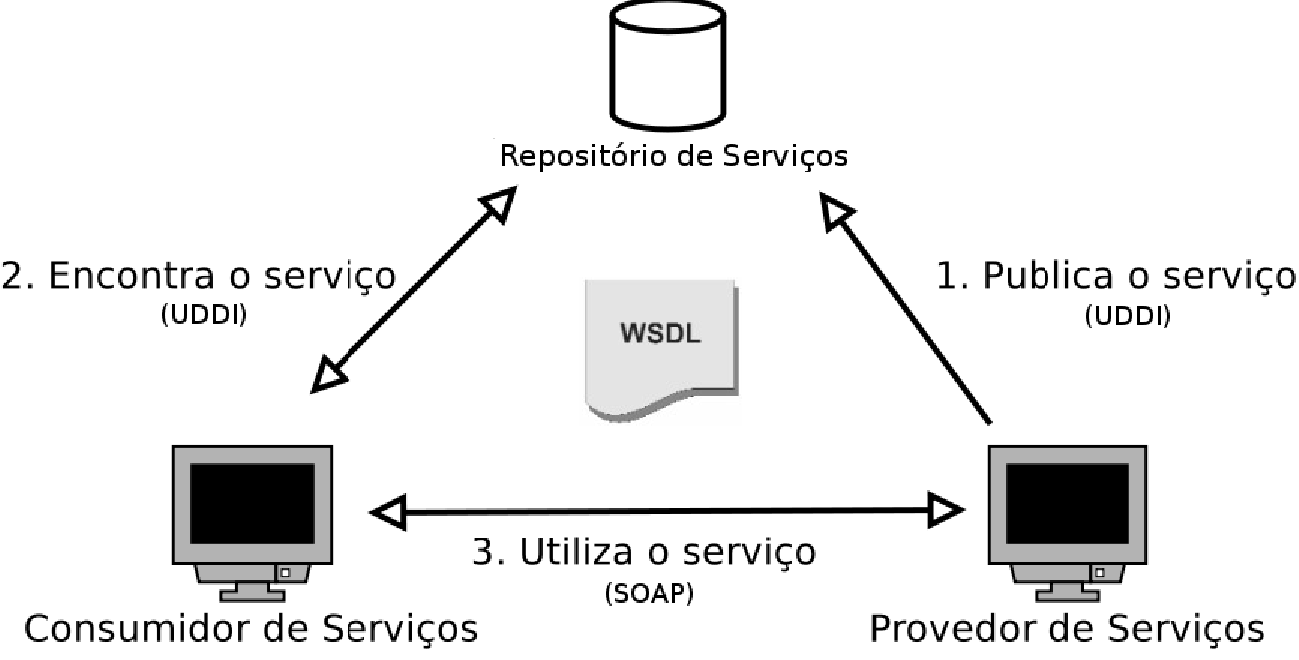
\includegraphics[scale=0.50]{imagens/SOA.pdf} 
		\caption{Padrões SOA estabelecidos.}
		\label{fig:SOA}
	    \end{center}
	    \end{figure}

	    \begin{figure}[!htb]
	    \begin{center}
		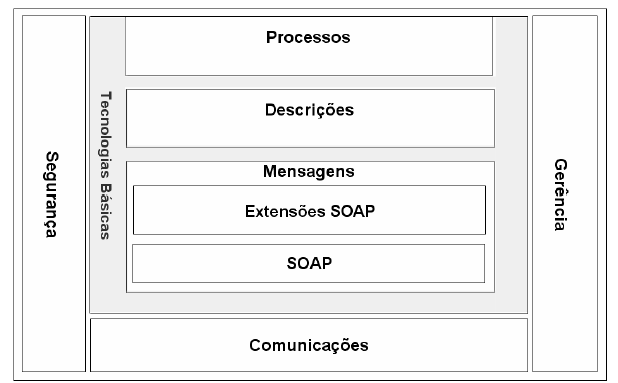
\includegraphics[scale=0.60]{imagens/ws.png} 
		\caption{Estrutura básica de um serviço Web.}
		\label{fig:WS}
	    \end{center}
	    \end{figure}             

	    \subsubsection{Descoberta: UDDI}
	    \label{subsec:UDDI}
		O padrão \textit{Universal Description, Discovery and Integration} (UDDI)~\cite{UDDI:website} oferece aos usuários de serviços Web, através de um registro centralizado equivalente a uma  ``lista telefônica'' online, um mecanismo para localizar provedores, os serviços disponibilizados por eles e as informações necessárias para acessá-los~\cite{IntroWS}.
		
		Baseado em XML, provê uma infraestrutura para integrar informação em ambientes de serviços Web tanto para serviços disponíveis publicamente quanto para serviços expostos internamente em organizações.
		O UDDI provê duas especificações básicas que definem a estrutura e operações do serviço de registro~\cite{IntroWS}:
		\begin{itemize}
		    \item uma definição das informações a serem fornecidas sobre cada serviço, e como codificá-las;
		    \item uma API de consulta e atualização do registro que descreve como a informação pode ser acessada ou atualizada.
		\end{itemize}
		
		Tanto a consulta quanto a atualização são realizadas através da troca de mensagens SOAP.

		As informações no repositório estão categorizadas de acordo com o objetivo de uso de cada tipo de informação, fazendo uma analogia com um diretório de telefones~\cite{alonso2004}:
		\begin{itemize}
		    \item \textbf{Páginas Brancas:} Listagens de organizações, informações de contato e serviços que elas provêem.
			    Usando o registro como um catálogo de páginas brancas, os usuários do UDDI podem encontrar serviços Web providos por uma dada empresa;
		    \item \textbf{Páginas Amarelas:} Classificações de organizações e WSs de acordo com taxonomias padrão ou definidas pelo usuário.
			    Através das páginas amarelas, é possível buscar serviços pela categoria a qual eles pertencem, de acordo com um dado esquema de classificação.
		    \item \textbf{Páginas Verdes:} Descrevem como um dado Serviço Web pode ser invocado;
			    Essa informação é obtida através de apontadores para a documentação do serviço, geralmente armazenada fora do registro (ex: Página da Web do provedor do serviço).
		\end{itemize}

		Inicialmente, o padrão UDDI foi projetado para apoiar um modelo conhecido como \textit{Universal Business Registry} (UBR)~\cite{IntroWS}, representando um serviço público e central.
		Entretanto, a maioria dos serviços Web da atualidade são ou internos a uma única instituição, ou compartilhado por alguns parceiros de confiança.
		Dessa forma, o padrão UDDI evoluiu na sua versão 3.0 para também apoiar registros privados.
		Os seguintes tipos de repositório são permitidos~\cite{alonso2004}:

		\begin{itemize}
		    \item \textbf{Repositório público:} repositório que provê acesso público e aberto aos dados de registro.
			    Um repositório disponível como um site na Web publicado e conhecido é um exemplo de repositório público;
		    \item \textbf{Repositório privado:} repositório interno, isolado por um \textit{firewall} de uma rede privada.
			    Organizações podem utilizar repositórios privados para apoiar a integração de suas próprias aplicações internas;
		    \item \textbf{Repositório compartilhado:} repositório instalado em um ambiente controlado, sendo compartilhado com um grupo limitado de organizações.
			    Por exemplo, uma rede de parceiros de negócio pode utilizar um repositório compartilhado para apoiar a integração de aplicações entre eles.
		\end{itemize}

	    \subsubsection{Descrição: WSDL}
		A \textit{Web Services Description Language} (WSDL)~\cite{WSDL} foi criada em conjunto pela IBM, Microsoft e Ariba através da união de especificações propostas individualmente por essas empresas. %TODO: REF de IBM M$ e Ariba?
		Seu objetivo principal é fornecer aos usuários a interface dos serviços Web, provendo um ponto de acesso para consumidores de serviços, informando quais mensagens devem ser trocadas para executá-los.
		Trata-se de um documento escrito em XML\footnote{\textit{Extensible Markup Language}} que além de descrever o serviço, especifica como acessá-lo e quais as operações ou métodos disponíveis~\cite{IntroWS}.
		
		Uma descrição WSDL completa inclui dois tipos de informação.
		Uma descrição de serviços no nível de aplicação, chamada de interface abstrata, e a descrição detalhada e dependente de protocolo, chamada de interface concreta~\cite{IntroWS}.
		%TODO: Pode explicar aqui porque separa e talz.. tem na mesma referência.
		A \autoref{fig:WSDL-est} mostra a estrutura de um documento WSDL contendo as interfaces concreta e abstrata.
				
		\begin{figure}[!htb]
		\begin{center}
		    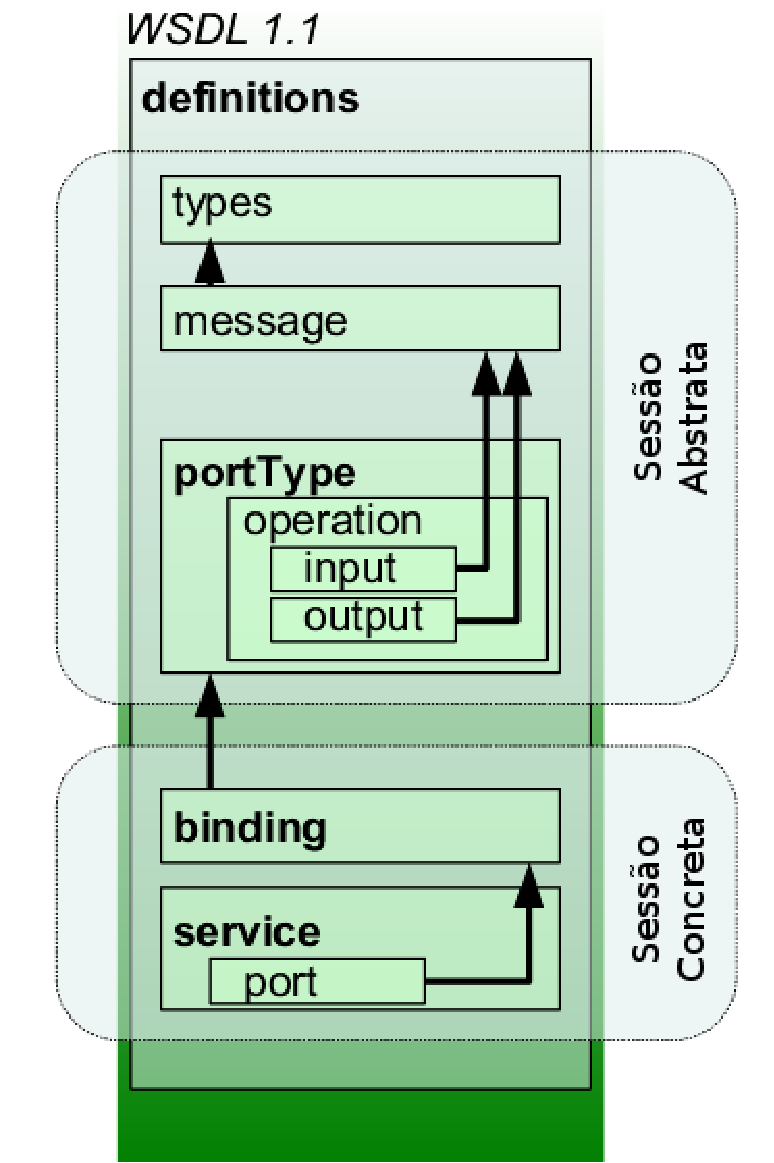
\includegraphics[scale=0.50]{imagens/wsdl-est.pdf} 
		    \caption{Estrutura WSDL 1.1.}
		    \label{fig:WSDL-est}
		\end{center}
		\end{figure}

		A parte abstrata de uma descrição de serviço WSDL é definida em termos de mensagens trocadas em uma interação com o serviço, compreendendo os seguintes elementos~\cite{marioLivro}:
		
		\begin{itemize}
		    \item \textbf{portType:} descreve uma coleção de operações oferecidas;
		    \item \textbf{operation:} descrição abstrata de uma ação que um determinado serviço pode oferecer. Define uma coleção de mensagens informando qual o papel de cada uma;
		    \item \textbf{types:} informa os tipos de dados empregados pelo serviço.
			    Geralmente utiliza-se o esquema de definição XML, também conhecido como XSD~\cite{xsd:website}.
		\end{itemize}

		Os elementos WSDL que compõem a parte concreta de uma descrição de serviço são apresentados a seguir~\cite{alonso2004}:

		\begin{itemize}
		    \item \textbf{binding:} especifica o estilo de interação e o protocolo de comunicação para um elemento \texttt{portType};
		    \item \textbf{port:} combina informações de ligação com um ponto de acesso, especificado por um URI através do qual uma implementação de um \texttt{portType} determinado pode ser acessada; %TODO: Ainda não expliquei o que é URI.
		    \item \textbf{service:} é uma coleção de elementos \texttt{port}.
		\end{itemize}
		
		O \autoref{cod:WSDL-ex} ilustra a utilização desses elementos em uma descrição de serviço Web.
		No exemplo de documento WSDL, um elemento \texttt{portType} (\texttt{Implementação}) define uma operação chamada \texttt{executar} (linhas~7-11).
		Essa operação inclui uma mensagem de entrada nomeada \texttt{executarMsg} (linha~9).
		Os componentes da mensagem são definidos utilizando o elemento \texttt{message} (linhas~3-5).
		Na parte concreta da descrição de serviço, um elemento \texttt{binding} é especificado para o \texttt{portType} definido na parte abstrata (linhas~14-21).
		O elemento binding \texttt{ImplementaçãoPortBinding} determina, por exemplo, a utilização de HTTP como protocolo de comunicações (linha~15).
		Finalmente, um serviço (\texttt{ImplementaçãoService}) é criado, definindo um elemento \texttt{port}, chamado \texttt{ImplementaçãoPort}, que combina o elemento \textit{binding} com o ponto de acesso de uma implementação do elemento \texttt{portType} definido anteriormente (linhas~23-27).
		

		%Exemplo WSDL
% 		\begin{figure}[!htb]
% 		    \centering
 		    \lstinputlisting[float=!htb,language=XML,
				    caption={[Exemplo WSDL 1.1.]Exemplo WSDL 1.1 contendo apenas as estruturas principais. Detalhes foram omitidos.},
				    label=cod:WSDL-ex]{listings/wsdl.xml}
% 		\caption[Exemplo WSDL 1.1.]{Exemplo WSDL 1.1 contendo apenas as estruturas principais. Detalhes foram omitidos.}
% 		\label{fig:WSDL-ex}
% 		\end{figure}

	    \subsubsection{Comunicação: SOAP}
	    
		O \textit{Simple Object Access Protocol} (SOAP) é um protocolo baseado em XML que possibilita a comunicação entre serviços Web.
		Ele define como deve ser o formato de uma mensagem trocada entre duas aplicações e utiliza protocolos já existentes para o envio das mensagens como, por exemplo, HTTP, SMTP~\cite{IntroWS}.
		
		A estrutura básica de uma mensagem SOAP é bem simples: um elemento XML principal, chamado de envelope, contendo uma área de cabeçalho e uma área para o corpo da mensagem.
		Essa estrutura pode ser vista na \autoref{fig:SOAP-est}.

		\begin{figure}[!htb]
		\begin{center}
		    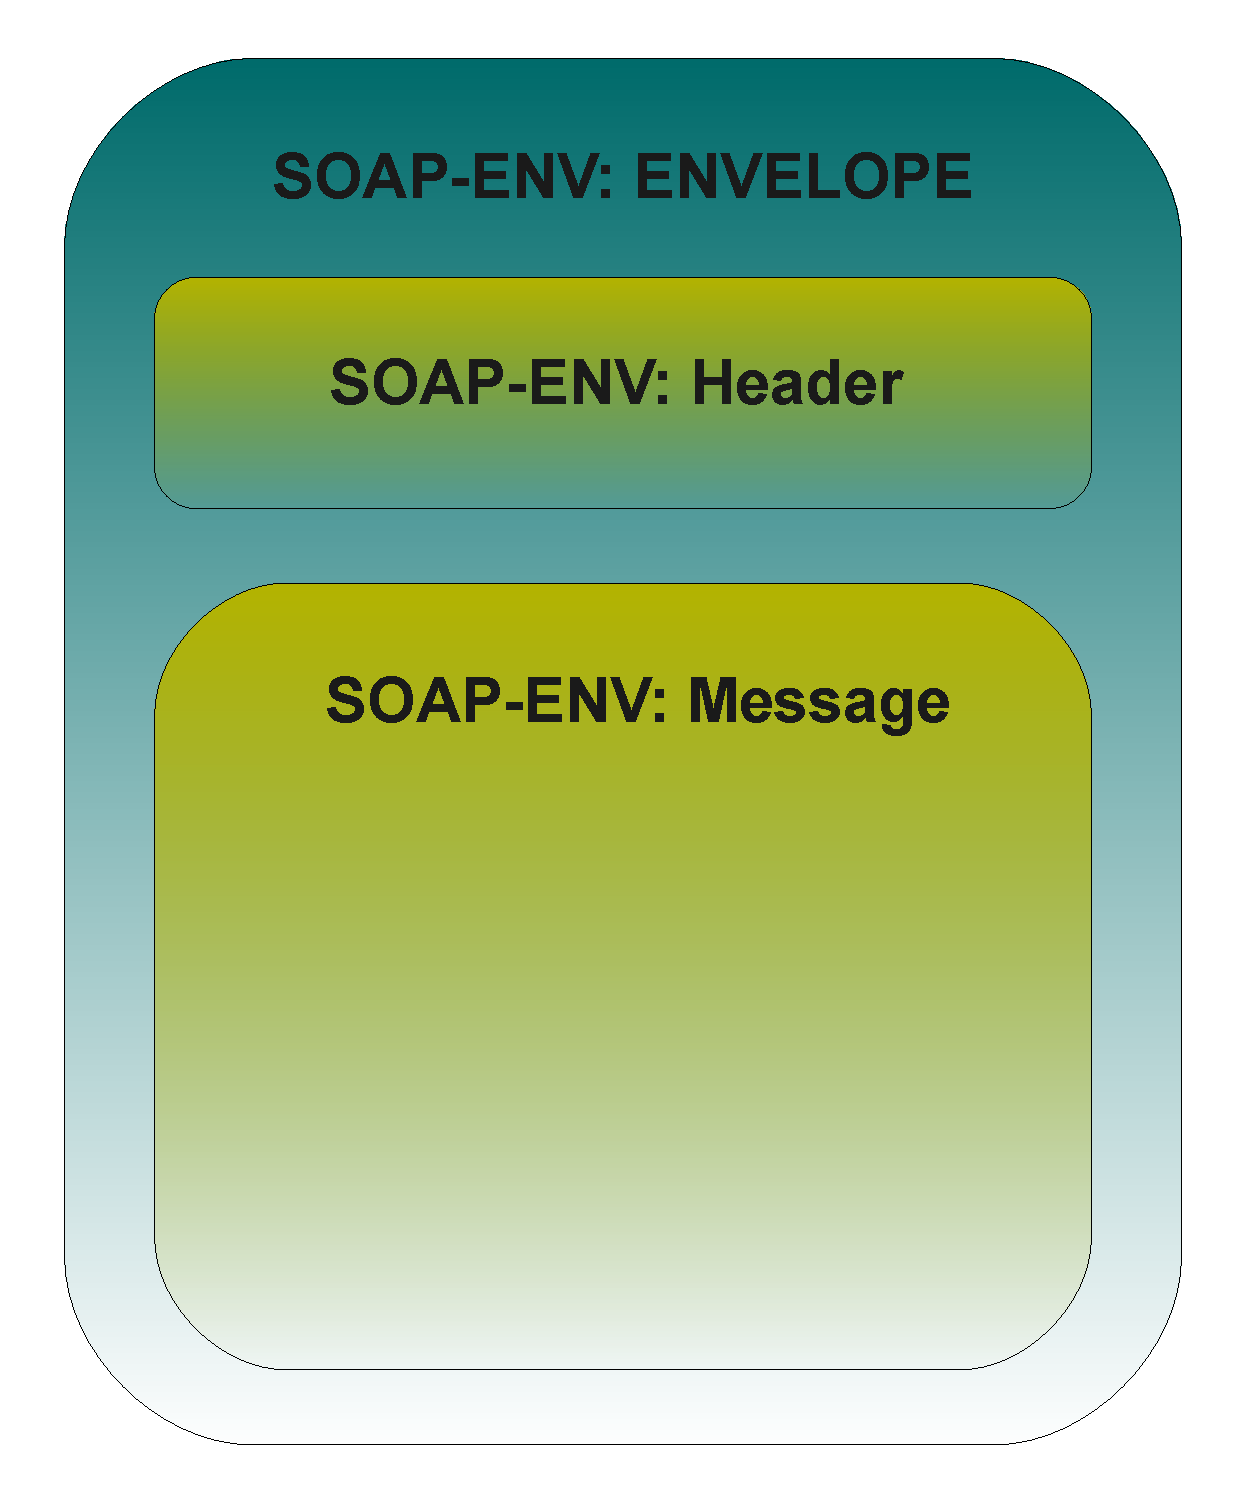
\includegraphics[scale=0.3]{imagens/SOAP-est.pdf} 
		    \caption{Estrutura de uma mensagem SOAP.}
		    \label{fig:SOAP-est}
		\end{center}
		\end{figure}

		O elemento \texttt{Header} é opcional e pode ser utilizado para funções específicas da aplicação no transporte da mensagem.
		Os intermediários através dos quais a mensagem passa entre a origem e o destino final podem processar esses cabeçalhos de maneira a implementar diversas funcionalidades como, por exemplo, autenticação, controle de transação, entre outros~\cite{LudwigWS}.
		
		Já o elemento \texttt{Body} contém a mensagem propriamente dita que está sendo trocada entre as aplicações.
		Esse corpo da mensagem pode implementar dois tipos de interação entre as aplicações~\cite{alonso2004}:
		
		\begin{itemize}
		    \item \textbf{Document-Style:} Nesse tipo de interação o elemento \texttt{Body} transporta uma mensagem XML que diz respeito a um documento que está sendo trocado entre as aplicações como, por exemplo, um pedido de compra contendo todos os itens, quantidade e preço.
		    Dessa forma, o serviço destino recebe essa mensagem e processa esse documento;
		    \item \textbf{RPC-Style:} Nesse tipo de interação o elemento \texttt{Body} transporta um documento que carrega informações sobre uma chamada de procedimento remoto, contendo qual procedimento deve ser invocado e o valor de cada um dos seus parâmetros.
		\end{itemize}
		
		O \autoref{cod:SOAP-ex} retrata um exemplo de mensagem SOAP.
		Primeiramente o \texttt{Envelope} é criado (linhas~1-17).
		Em seguida, o \textit{Header} é definido (linhas~3-8) com os parâmetros \textit{MessageID} (linha~4) e \textit{ReplyTo} (linhas~5-7).
		Finalmente o corpo da mensagem é criado (linhas~10-15) para invocar a operação \texttt{executar} (linhas~11-14), e informando os parâmetros \texttt{comando} (linha~12) e \texttt{arqOutput} (linha~13).
		Essa mensagem SOAP foi criada para invocar o serviço definido no WSDL demonstrado anteriormente no \autoref{cod:WSDL-ex}.

		%Exemplo SOAP
% 		\begin{figure}[!htb]
% 		    \centering
 		    \lstinputlisting[float=!htb,language=XML,
				    caption={[Exemplo de uma mensagem SOAP.]Exemplo de uma mensagem SOAP contendo apenas as estruturas principais. Detalhes foram omitidos.},
				    label=cod:SOAP-ex]{listings/soap.xml}
% 		\caption[Exemplo de uma mensagem SOAP.]{Exemplo de uma mensagem SOAP contendo apenas as estruturas principais. Detalhes foram omitidos.}
% 		\label{fig:SOAP-ex}
% 		\end{figure}

%%%%%%%%%%%OUTROS%%%%%%%%%%%%%%%%%%
	\subsection{Outros Padrões Relacionados}
	    Existem diversos outros padrões associados à arquitetura orientada a serviços e os WSs.
	    Nessa subseção serão apresentados os mais relevantes a este trabalho.           
      
	    \subsubsection{WS-Addressing}
		\label{section:WS-Addressing}
		WS-Addressing~\cite{wsad:website} é uma especificação para permitir que serviços Web comuniquem informações de endereçamento.
		É uma maneira padronizada de incluir informações de roteamento da mensagem no cabeçalho de mensagens SOAP~\cite{alonso2004}.
		
		Essa especificação é comumente utilizada para a comunicação de serviços Web em modo assíncrono. 
		Através da configuração da \textit{tag} \texttt{ReplyTo} no cabeçalho WS-Addressing, o provedor do serviço pode responder à mensagem através de uma nova conexão.
		Dessa forma, o tempo de vida da chamada/resposta SOAP fica desacoplado do tempo de vida do protocolo HTTP, permitindo a execução de processos muito demorados~\cite{alonso2004}.
		
		Os principais elementos de um cabeçalho WS-Addressing são:
		
		\begin{itemize}
		    \item \textbf{MessageID:} Código usado para identificar unicamente a mensagem;      
		    \item \textbf{ReplyTo:} Endereço para qual o serviço deve enviar a resposta;
		    \item \textbf{RelatesTo:} Utilizado nas mensagens de resposta, contém o mesmo valor do \textit{MessageID} da mensagem original.
		    É através desse valor que o cliente pode associar as requisições às respostas.
		\end{itemize}
		
		Ainda no \autoref{cod:SOAP-ex} é possível verificar a utilização do WS-Addressing no cabeçalho (linhas~3-8).
		A mensagem de resposta deverá ser destinada ao endereço contido na \textit{tag} \texttt{ReplyTo}, e deverá conter a \textit{tag} \texttt{RelatesTo} com o mesmo valor do \textit{MessageID} de entrada, de forma similar ao \autoref{cod:Addressing}.

		%Exemplo WS-Addressing
% 		\begin{figure}[!htb]
% 		    \centering
		    \lstinputlisting[float=!htb,language=XML,
				    caption={Trecho do cabeçalho de uma requisição SOAP de resposta utilizando WS-Addressing.},
				    label=cod:Addressing]{listings/addressing.xml}
% 		\caption{Trecho do cabeçalho de uma requisição SOAP de resposta utilizando WS-Addressing.}
% 		\label{fig:Addressing}
% 		\end{figure}
      
	    \subsubsection{WS-Policy}
		Embora WSDL seja o padrão para a descrição de funcionalidade de serviços Web, esforços de pesquisas recentes estão focados em linguagens que possam aprimorar tal descrição.
		Esse aprimoramento inclui a consideração de aspectos que não são diretamente relacionados com o que um serviço faz ou como invocar um serviço Web.
		O \textit{Web Services Policy Framework} (WS-Policy)~\cite{wspolicy:website} representa um desses esforços e, devido à sua flexibilidade e capacidade de extensão, é um candidato para tornar-se um padrão para a especificação de políticas para serviços Web~\cite{Baresi06ws}.
		
		O WS-Policy é apoiado por um consórcio formado por diversas empresas, como, por exemplo, BEA, IBM, Microsoft, SAP e VeriSign.
		Esse consórcio foi responsável pela submissão de especificações nas áreas de transações, confiabilidade de mensagens, dentre outras, para entidades de padronização de serviços Web.
		
		O padrão compreende um modelo para definir propriedades de serviços Web e uma sintaxe correspondente para expressar essas definições como políticas.
		Referências para políticas podem ser incluídas em documentos XML~\cite{wspolicyattachment:website}.
		Políticas podem ser aplicadas em diferentes níveis, tais como, mensagem, operação e serviço.
		
		Em WS-Policy, uma política é uma coleção de alternativas.
		Cada alternativa de política é uma coleção de asserções.
		Tipicamente, asserções de política especificam características que são importantes para a seleção e utilização apropriadas de serviços Web, por exemplo, características não-funcionais~\cite{wspolicy:website}.
		
		O padrão WS-Policy define um formato normalizado para especificar políticas com o objetivo de facilitar sua manipulação.
		A forma normal de política WS-Policy é uma disjunção das alternativas de uma política e uma conjunção das asserções em cada uma das alternativas da política.
		
		Alguns exemplos de atributos de QoS são descritos a seguir:
		\begin{itemize}
		    \item \textbf{Tempo de resposta:} O intervalo de tempo demandado para que um serviço complete sua tarefa;
		    \item \textbf{Capacidade:} O número de requisições concorrentes permitido por um serviço;
		    \item \textbf{Disponibilidade:} A porcentagem de tempo em que um serviço está operante;
		    \item \textbf{Segurança:} Define se um serviço oferece mecanismos de confidencialidade, integridade, autenticação e autorização.
		\end{itemize}     	

		O \autoref{cod:WSPolicy} apresenta um exemplo de um WS-Policy.
		A política define que tempo de resposta (\texttt{ResponseTime}) para a operação \texttt{get} deve ser menor que \texttt{45} (linha~8).
		A \textit{tag} \texttt{wsp:All} indica que todas as políticas devem ser atendidas (linha~3).


		%Exemplo WS-Policy
% 		\begin{figure}[!htb]
% 		    \centering
 		    \lstinputlisting[float=!htb,language=XML,
				    caption={[Exemplo de uma política WS-Policy.]Exemplo de uma política WS-Policy contendo apenas as estruturas principais. Detalhes foram omitidos.},
				    label=cod:WSPolicy
				    ]{listings/policy-qos.xml}
% 		\caption[Exemplo de uma política WS-Policy.]{Exemplo de uma política WS-Policy contendo apenas as estruturas principais. Detalhes foram omitidos.}
% 		\label{fig:WSPolicy}
% 		\end{figure}

	    %TODO: Falta falar do WS-Policy - Attachment


    \section{Orquestração de serviços}

	A computação distribuída tem rumado para uma arquitetura orientada a serviços em que funções computacionais são representadas por serviços Web.
	Essa abordagem abre a possibilidade de se criar novos serviços combinando outros serviços existentes.
	Dessa forma, a reusabilidade de recursos existentes entra em cena e novas funcionalidades podem ser implementadas de maneira mais rápida.

	A orquestração é criada através da definição de um ``processo de negócio'' que capta a lógica de como os serviços individuais devem ser combinados.
	Essa abordagem atrai um grande interesse tanto da indústria quando da academia~\cite{Tan06}.

	Serviços Web podem ser combinados de diferentes maneiras para formar uma composição de serviços.
	Os principais modos são: sequencial, paralela e com escolha.
	Na composição sequencial um segundo serviço só será invocado depois que o primeiro terminar a sua execução.
	Na composição com escolha apenas um serviço é escolhido para ser executado dependendo de um critério previamente especificado.
	Por fim, na composição paralela, diversos serviços são executados de maneira simultânea.

	Uma orquestração pode ser representada através de um \textit{workflow}, que pode conter os três tipos citados anteriormente.
	No contexto dos serviços Web, um grande avanço veio do desenvolvimento do WS-BPEL (\textit{Web Services Business Process Execution Language}), que agora está estabelecida como a maneira padrão de os compor~\cite{Tan06}.


	\subsection{Workflow}
	
	    A história dos \textit{workflows} começou ainda no fim dos anos 70 quando estes despertaram atração pela habilidade de descrever um processo de uma maneira simples de entender, modificar, executar e monitorar.
	    A \textit{Workflow Management Coalition} (WfMC)~\cite{wfmc:website} define um \textit{workflow} como a automação de um processo de negócio, ou parte dele, cujos documentos, informações ou tarefas são passadas de um participante para outro para serem processados, de acordo com um grupo de regras~\cite{Slomiski06}.

	    Os sistemas baseados nessa ideia podem ser classificados em uma escala com três níveis~\cite{FOX06}: Simples e linear, grafos acíclicos e grafos cíclicos.
	    O primeiro tipo é caracterizado por uma sequência de tarefas em uma ordem linear, em que a primeira tarefa transforma um objeto de dados iniciais em um novo objeto que irá servir de entrada para a próxima tarefa e assim sucessivamente.
	    O segundo nível é formado por um grafo acíclico, cujos nós representam as tarefas a serem executadas e as arestas a dependência entre tarefas.
	    O último tipo é similar ao anterior, porém possui ciclos que representam, de forma implícita ou explícita, uma repetição ou um mecanismo de controle de iterações.

	    Os principais componentes de um \textit{workflow} podem ser definidos da seguinte maneira:
	    
	    \begin{itemize}
		\item \textbf{Processo:} Um processo é um conjunto de um ou mais procedimentos interdependentes que, coletivamente, cumprem um objetivo.
			A divisão entre processos de negócio e processos científicos é comum, diferenciados pelo contexto em que estão inseridos.
			Respectivamente: envolvendo trocas comerciais e/ou monetárias; e executando experimentos científicos;

		\item \textbf{Atividade:} Uma descrição de uma parte do trabalho a ser realizado em um processo.
			Uma atividade pode ser básica (ou atômica), ou pode ser um subfluxo, composto de outras atividades.
			Atividades são os elementos básicos da construção de \textit{workfows};
						    
		\item \textbf{Sistema Gerenciador de Workflows (SGWf):}  Um sistema automatizado para definir e instanciar \textit{workfows}, e gerenciar sua execução.
			Essa execução pode ocorrer em uma ou mais máquinas de execução, que são capazes de interpretar as definições de um \textit{workfow} e interagir com os seus participantes.
	    \end{itemize}            
				    
	    Para sistemas grandes, ou para \textit{workflows} de estruturas mais complexas e dinamicamente estruturadas, é necessário algo que se assemelhe a uma linguagem de programação completa, e WS-BPEL é uma das candidatas para esse propósito~\cite{FOX06}.
                           
	\subsection{WS-BPEL}
	\label{subsec:BPEL}
	    A linguagem WS-BPEL~\cite{bpel:website}, \textit{Web Services Business Process Execution Language}, é um padrão criado pela OASIS (\textit{Organization for the Advancement of Structured Information Standards}) para a execução de processos de negócio, descrevendo como ocorre o relacionamento entre os diversos serviços Web participantes da composição.
	    Trata-se de uma linguagem baseada em XML que descreve um \textit{workflow} de serviços~\cite{MargolisSOA}.
				    
	    BPEL herdou as características de linguagens anteriores como WSFL da IBM e XLANG da Microsoft e está disponível na versão 2.0.
	    A estrutura principal de um processo de negócio especificado em WS-BPEL é formada por três seções: \texttt{PartnerLinks}, \texttt{Variables} e \texttt{Activities}.
	    Cada uma dessas sessões será discutida posteriormente.

	    Um processo BPEL executa um \textit{workflow} primariamente acessando um serviço após o outro, conforme a ordem definida na composição. 
	    Cada um desses serviços é chamado de \texttt{partner service}.

	    Cada atividade (\texttt{activity}) é equivalente a uma chamada de função em uma linguagem de programação.
	    A atividade do tipo \texttt{receive} aguarda uma mensagem de entrada, e a atividade do tipo \texttt{invoke} transmite uma mensagem, geralmente executando um serviço.  
	    
	    O \autoref{cod:BPEL-ex} retrata um exemplo de \textit{workflow} descrito na linguagem WS-BPEL.
	    Podemos identificar as seguintes etapas:
	    
	    \begin{enumerate}
		\item Criação dos \texttt{partner links}, que fornecem detalhes sobre a relação entre os processo BPEL e cada \texttt{partner service} (linhas~2-4);
		\item Atribuição de variáveis, que serão utilizadas durante a execução do processo (linhas~6-9);
		\item A criação de uma atividade estruturada do tipo \texttt{sequence}, contendo outras atividades (linhas~11-22);
		\item O recebimento de uma chamada a função \texttt{OperationA} através da uma operação simples do tipo \texttt{receive} (linha~12);
		\item Atribuição de valores as variáveis criadas anteriormente através a operação \texttt{assign} (linhas~14-19);
		\item Chamada da operação externa \texttt{execSharcnet} através da operação \texttt{invoke} (linha~21).
	    \end{enumerate}

	    %Exemplo WS-BPEL
% 	    \begin{figure}[!htb]
% 		\centering
 		\lstinputlisting[float=!htb,language=XML,
				caption={[Exemplo de um \textit{workflow} descrito na linguagem BPEL.]Exemplo de um \textit{workflow} descrito na linguagem BPEL. Detalhes foram omitidos.},
				label=cod:BPEL-ex]{listings/bpel.xml}
% 	    \caption[Exemplo de um \textit{workflow} descrito na linguagem BPEL.]{Exemplo de um \textit{workflow} descrito na linguagem BPEL. Detalhes foram omitidos.}
% 	    \label{fig:BPEL-ex}
% 	    \end{figure}

	    \subsubsection{PartnerLinks}
		Seção que define os diferentes parceiros (partes envolvidas) que interagem com o processo de negócio durante toda sua execução.
		Eles são usados para identificar a funcionalidade que deve ser oferecida por cada serviço parceiro.
		As ligações de parceiros (\texttt{partner link}) devem estar associadas a um tipo de ligação entre parceiros (\texttt{partner link type}) definido na especificação de serviços Web em WSDL.

	    \subsubsection{Variables}
		Seção que define as variáveis de dados usadas pelo processo de negócio.
		As definições são feitas em termos de tipos de mensagem WSDL, elementos ou tipos simples de esquemas XML.
		Elas são usadas para manter os dados de estado e o histórico do processo com base nas mensagens trocadas.
		As variáveis devem estar associadas a tipos de mensagens (\texttt{messages}) definidos na especificação WSDL.

	    \subsubsection{Activities}
		Seção que contém a descrição do comportamento normal para a execução do processo de negócio.
		Existem basicamente dois tipos de atividades, as atividades básicas (\texttt{Basic Activities}) e as atividades estruturadas (\texttt{Structured Activities}).
		
		Uma \texttt{Basic Activity} é um tipo de atividade usado para executar alguma operação.
		Algumas dessas atividades básicas envolvem a interação com algum parceiro, como: \texttt{invoke}, \texttt{receive} e \texttt{reply}.
		Outras dessas atividades são executas sem a interação com qualquer parceiro, como: \texttt{wait}, \texttt{terminate}, \texttt{assign}, \texttt{empty}, \texttt{throw} e \texttt{compensate}.

		Uma \texttt{Structured Activity} é um tipo de atividade usado para agrupar atividades básicas dentro de algumas estruturas de fluxo.
		Tais atividades são: \texttt{while}, \texttt{pick}, \texttt{flow}, \texttt{sequence}, \texttt{switch} e \texttt{scope}.

	    \subsubsection{Execução de serviços assíncronos}
		A chamada de um serviço pode ser tanto de forma síncrona quando de forma assíncrona, sendo os dois métodos definidos pela estrutura \textit{invoke} da linguagem BPEL.
		Chamadas que incluem tanto variáveis de entrada quanto de saída são executadas de forma síncrona e o \textit{workflow} BPEL é bloqueado enquanto o serviço executa.
		Para execuções assíncronas, o BPEL fornece a notação de grupos de correlação (\texttt{Correlation Sets}) que são utilizados para associar \texttt{invokes}, contendo somente variáveis de saída, com seus respectivos \texttt{replies}, contendo as variáveis de entrada ~\cite{Emmerich05}.

		O solicitante de um serviço assíncrono inicia a interação invocando uma operação de direção única no provedor.
		Quando o provedor termina a execução, ele retorna o resultado invocando outra operação de direção única no solicitante, conhecida como \textit{callback}.
		O endereço do de resposta do solicitante e os valores utilizados para criar a correlação são enviados do cabeçalho das mensagens utilizando o WS-addressing, explicado anteriormente na \autoref{section:WS-Addressing}.
		O provedor utiliza, então, o grupo de correlação para especificar qual instância de processo a mensagem de \textit{callback} se refere~\cite{Emmerich05}.

		A \autoref{fig:BPEL-assinc} retrata um diagrama de interação demonstrando um exemplo de um processo WS-BPEL executando um serviço Web de forma assíncrona.
		As seguintes ações podem ser vistas:
		
		\begin{enumerate}
		    \item No processo BPEL, uma atividade do tipo \texttt{invoke} inicia um serviço montando uma mensagem SOAP;
		    \item Um cabeçalho WS-addressing é adicionado à mensagem SOAP, informando o endereço do serviço que aguarda a mensagem de \textit{callback}, e o identificador de correlação;
		    \item Usando a descrição WSDL do serviço, uma porta é iniciada e os dados para o serviço assíncrono são enviados;
		    \item O serviço assíncrono processa a requisição e envia uma resposta de volta ao processo BPEL através de uma porta de \textit{calback}.
			O cabeçalho WS-addressing é montado com o identificador de correlação apropriado (o mesmo da mensagem \texttt{invoke});
		    \item A máquina de composição BPEL verifica o identificador de correlação na mensagem de \textit{callback} e identifica a instância que a aguardava.
		\end{enumerate}
		
		\begin{figure}[!htb]
		\begin{center}
		    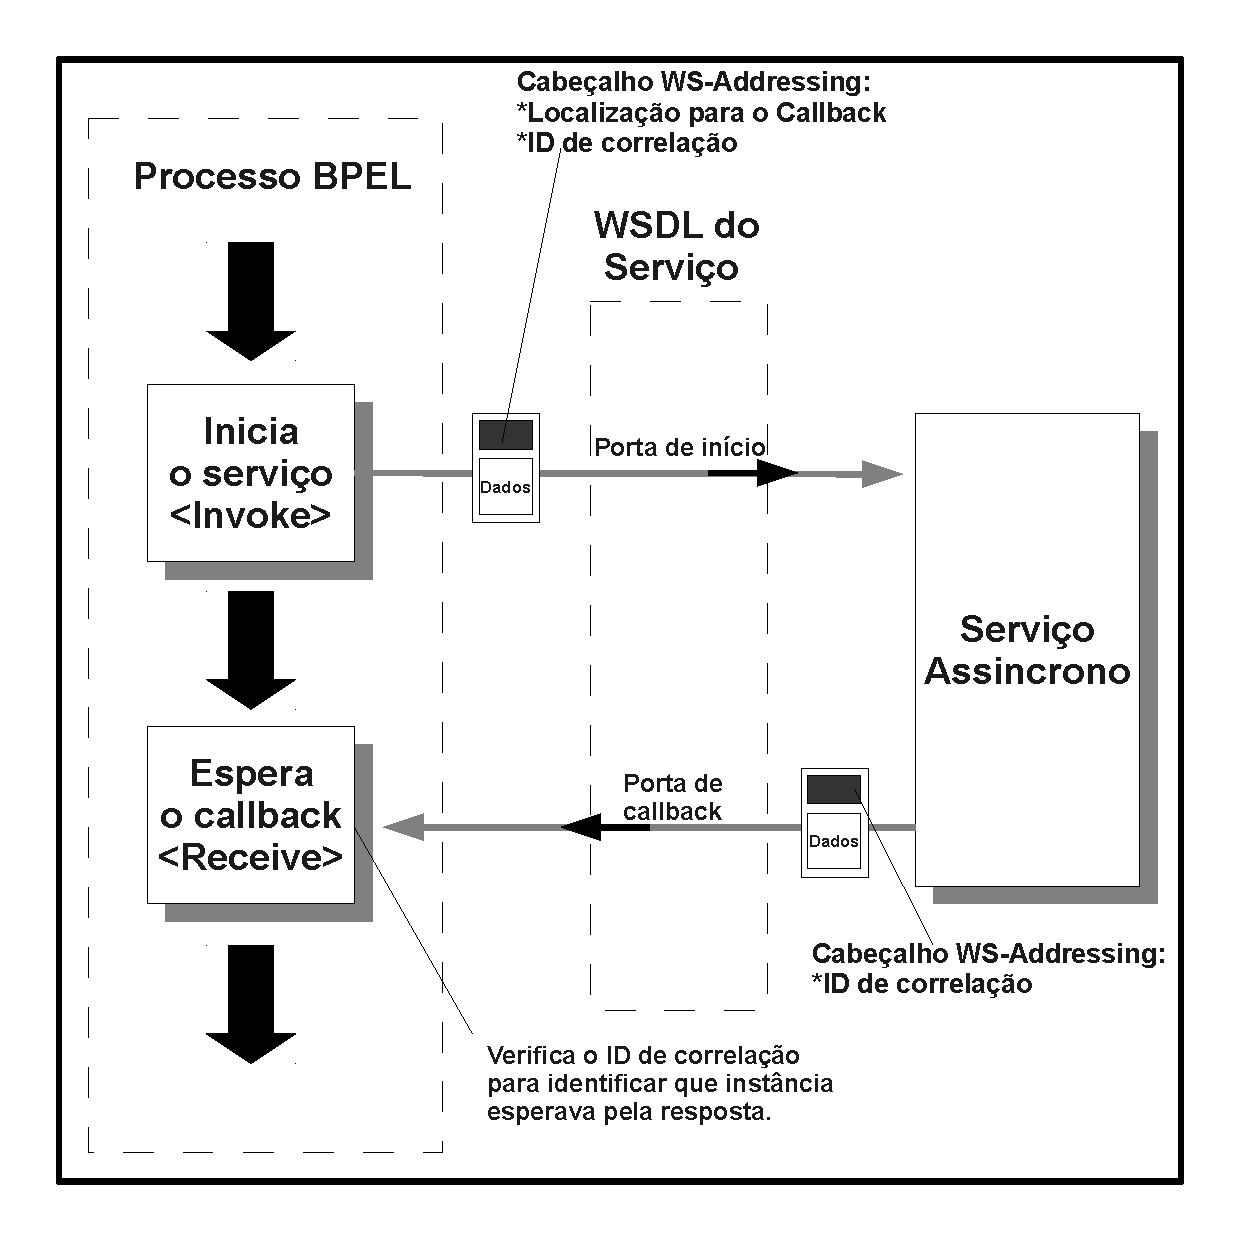
\includegraphics[scale=0.50]{imagens/bpelassinc.pdf}
		    \caption{Diagrama de interação de um processo WS-BPEL executando um serviço Web de forma assíncrona.}
		    \label{fig:BPEL-assinc}
		\end{center}
		\end{figure}
		

	\subsection{WS-BPEL e os Multi-Clusters}
	    Pesquisas recentes sugerem a integração de duas tecnologias existentes, \textit{workflows} e sistemas distribuídos, como uma solução para problemas que são ao mesmo tempo complexos e necessitam de um grande poder computacional.

	    Os \textit{workflows} têm sido revistos para aplicações, científicas e comerciais, de alta intensidade que executam em sistemas distribuídos, como \textit{Multi-Clusters} ou grades computacionais.
	    Apesar de diversos serviços, incluindo autenticação, gerenciamento, descoberta e acesso a recursos remotos, estarem disponíveis aos desenvolvedores de aplicações distribuídas, esses serviços não são suficientes para resolver problemas complexos.
	    Nesse caso, os serviços precisam ser compostos e executados de forma simples, levando em consideração suas dependências.
	    A necessidade de se representar \textit{workflows} científicos e comerciais em sistemas distribuídos já foi destacada por diversos pesquisadores~\cite{Laszewski04, Buyya2005}, e a inadequações dos conceitos e padrões existentes foi reconhecida pelo \textit{Global Grid Forum}~\cite{FOX06}.

	    Visto que os serviços Web foram adotados na infraestrutura desses sistemas heterogêneos, WS-BPEL, o padrão para composição de serviços, é um forte candidato para a especificação de \textit{workflows} complexos~\cite{Khalaf06}.
	    O WS-BPEL provê um processo abstrato para a descrição de interações entre parceiros de negócio, além de tratamento de falhas e exceções, com uma linguagem para a definição da lógica de um processo executável em termos de Serviços Web e dados em XML~\cite{FOX06}.
	    
	    Além do mais, WS-BPEL é vantajoso por existirem máquinas de execução, comerciais e de código aberto, disponíveis para a interpretação e execução dos \textit{workflows}, facilitando a interoperabilidade.
	    Leymann~\cite{Leymann06} sugere que o WS-BPEL deve ser estendido aos ambientes distribuídos ao invés de criar-se um novo padrão.
	    Entretanto, o fluxo de atividade dessas arquiteturas possuem requisitos específicos, como gerenciamento de ciclo de vida e a seleção de recursos baseada em requisitos não-funcionais~\cite{krishnan02gsfl}.

\chapter{Trabalhos Relacionados}
\label{chap:RelatedWork}
    Neste capítulo serão discutidos  os principais trabalhos relacionados à presente dissertação.
    Primeiramente são levantados os trabalhos com o foco na execução de \textit{workflows} em sistemas distribuídos heterogêneos.
    Em seguida algumas pesquisas sobre escalonamento global em \textit{Multi-Clusters} são apresentadas.

    Como o intuito manter este trabalho sucinto, na \autoref{sec:RelatedWF} serão relacionados apenas os trabalhos que utilizam a linguagem WS-BPEL para expressar os \textit{workflows}.
    Contudo, também existem pesquisas com objetivos similares mas direcionadas a criação de novas linguagens~\cite{krishnan02gsfl,Tsalgatidou06,Dieter06}.
    Outro ponto importante é o fato de a grande maioria dos trabalhos utilizarem como infraestrutura grades computacionais.
    Até a data de escrita deste trabalho não foram encontradas pesquisas que tivessem um \textit{Multi-Clusters} como infraestrutura alvo.

    Apesar de não ser objetivo primário deste trabalho, criar um escalonador global funcional teve grande importância.
    Na \autoref{sec:RelatedEscalonador} são listados os trabalhos com esse intuito.



%   ---BPEL---
%   Slomiski06			- On using BPEL extensibility to implement OGSI and WSRF Grid workflows
%   Leymann06 			- Choreography for the Grid: towards fitting BPEL to the resource framework
%   Emmerich05 			- Grid Service Orchestration using the Business Process Execution Language(BPEL)
%   GridServiceComposition08 	- Grid Service Composition in BPEL for Scientific Applications  
%   GridEnabledWF08		- Grid-Enabled Workflow Management System Based On BPEL
%   
% 
% 
%   ---Não BPEL---
%   *Tsalgatidou06			- Developing scientific workflows from heterogeneous services
%   *Dieter06 [Cybok 2006]		- A Grid workflow infrastructure
%   *krishnan02gsfl
%   Triana [Taylor 2003, Majithia 2004]

    \section{Execução de Workflows em Sistemas Distribuídos Heterogêneos}
    \label{sec:RelatedWF}
	Como serviços Web já foram adotados nas infraestruturas de sistemas distribuídos e como BPEL oferece os requisitos de interoperabilidade, e permite o uso de máquinas de \textit{workflow} disponíveis, open-source ou industriais, ela é candidata a ser adotada também na comunidade de grades~\cite{Khalaf06}.
	Leymann~\cite{Leymann06} sugere que BPEL seja estendida para esses sistemas ao invés de se criar um novo padrão.
	Contudo, fluxos de atividades para aplicações desse tipo de infraestruturas resultam em requisitos específicos~\cite{Leymann06}. 

	WS-BPEL é utilizado em diversos projetos~\cite{Emmerich05,GridServiceComposition08,Leymann06,GridEnabledWF08,Slomiski06}.
	De fato, a maioria dos autores concorda que a WS-BPEL, com algumas modificações, pode e deve ser adotada para a composição de serviços de grade.
	Até mesmo autores que não a utilizam, como Cybok~\cite{Dieter06}, reconhecem sua importância a consideram como opção em pesquisas futuras.
  
	\subsection{Leymann}
	    Leymann~\cite{Leymann06} discute como os requisitos específicos de grades podem ser cumpridos pela linguagem BPEL.
	    Alguns dos requisitos discutidos são: tempo de vida e propriedades dos recursos, monitoramento e tratamento de transações.
	    
	    O autor discute extensivamente as vantagens e desafios para a utilização do BPEL em sistemas distribuídos heterogêneos e conclui que a comunidade de grades deve considerar o BPEL como base para composições ao invés de criar novas linguagens.
	    Segundo o autor, hoje a linguagem BPEL está perto de atender os requisitos para a execução de \textit{workflows}  em grades, precisando apenas de novas funcionalidades como, por exemplo, monitoramento.

	    %Se relaciona porque eh o precursor, e diz que dá pra fazer.

	\subsection{Slomiski}
	    Slomiski~\cite{Slomiski06} discute os benefícios e desafios no uso de BPEL em ambientes de grade.
	    O autor descreve suas experiências na tentativa de verificar se essa linguagem pode ser utilizada para facilitar a execução de \textit{workflows} grades OGSI, \textit{Open Grid Services Infrastructure}, e WSRF, \textit{Web Services Resource Framework}, (Tipos de arquitetura mais utilizadas em grades computacionais) e as compara.
	    Vale ressaltar que esse trabalho se limitou a usar uma linguagem existente, no caso o BPEL, e trabalhar somente com o que ela já disponibilizava, sem acrescentar nenhum tipo de funcionalidade.
	    
	    Inicialmente o trabalho discute como a linguagem BPEL pode ser integrada com uma grade baseada em OGSI.
	    Levanta divergências entre as especificações e propõe como solução para alguns dos problemas a criação de um \textit{proxy}.

	    Em seguida, o trabalho discute a integração da linguagem BPEL com uma grade baseada em WSRF.
	    Por ser uma especificação mais recente e mais direcionada aos serviços Web, a integração se torna muito mais simples.
	    Entretanto, algumas dificuldades ainda foram encontradas.
	    Entre elas, o autor destaca a dificuldade de se criar mecanismos de notificação e monitoramento.

	    Ao fim do trabalho, o autor argumenta que BPEL pode cumprir os requisitos para a execução de \textit{workflows} em grades com algumas adaptações para OGSI e WSRF.  

	    %Relaciona por causa da ideia do proxy
  
	\subsection{Emmerich et al.}
	    Em seu trabalho Emmerich et al.~\cite{Emmerich05} descrevem suas experiências na orquestração de \textit{workflows} científicos usando BPEL, obtidas durante um estudo de caso compondo serviços de grade.
	    Seus objetivos eram mostrar em que medida BPEL pode ser usado para a orquestração e descobrir se o mesmo é expressivo o suficiente para \textit{workflows} científicos.
	    
	    Primeiramente foi escolhido um problema representativo para o estudo de caso.
	    Foi escolhido um \textit{workflow} científico da área de teoria química, mais especificamente predição computacional de estruturas de cristais orgânicos a partir de um diagrama químico.
	    Em particular, o estudo replicou um experimento que foi codificado manualmente e executado em um servidor comum, codificando-o em BPEL e o executando em uma grade computacional.

	    Em seguida, foi utilizada a ferramenta ActiveBPEL para definir e executar o \textit{worflow} e foram medidos o desempenho, escalabilidade e confiabilidade da solução.

	    Nesse trabalho também foi discutido como derivar os requisitos para uma composição de serviços de grade e como BPEL trata cada um deles.
	    Os principais desses requisitos são:
	    \begin{itemize}
	    \item \textbf{Definição:} Invocar serviços de grades, controlar fluxo de controle e de dados, permitir composição hierárquica e tratamento de falhas;
	    \item \textbf{Implantação:} Possibilitar testes e implantação dos \textit{workflows};
	    \item \textbf{Execução:} Tratar de concorrência, escalabilidade e monitoramento.
	    \end{itemize}

	    Concluiu-se então que, em resumo, BPEL satisfaz a maioria desses requisitos.
	    Já que foi possível expressar a aplicação do estudo de caso por completo.
	    Contudo, os resultados não foram tão bons quanto poderiam.
	    Foi verificado que a linguagem poderia ser mais expressiva, pois acabou se tornando muito difícil para ser interpretada e modificada por humanos, e com um excesso de informação redundante.
	    Além de ser uma linguagem muito complexa, prejudicando a usabilidade e tornando uma ferramenta gráfica acessório necessário.
		
	    %Bem completo, estudo de caso e resultados para wf cientifico.

	\subsection{Ezenwoye et al.}
	    Em sua pesquisa, Ezenwoye et al.~\cite{GridServiceComposition08} demonstram experiências utilizando BPEL para integrar, criar e gerenciar recursos de grades baseadas em WSRF e que implementam um padrão de fábrica de objetos.
	    O autor apresenta um trabalho similar ao de Emmerich, entretanto utiliza um tipo diferente de aplicação, nesse caso uma aplicação de bioinformática para mapeamento de sequências de proteínas.
	    
	    O autor destaca problemas com a transferência de dados e demonstra os principais pontos de ajustes.
	    Como conclusão obteve-se sucesso na orquestração sendo o primeiro trabalho a incluir a descoberta de serviços.

	\subsection{Ma et al.}
	    Em Ma et al.~\cite{GridEnabledWF08} os autores têm como objetivo projetar e implementar um sistema de gerenciamento de \textit{workflows} baseados em BPEL em um sistema de grade.
	    Sua ideia principal é integrar a linguagem BPEL com um sistema WSRF através da implementação de um protótipo.
	    
	    Esse trabalho define uma sequência de atividades para invocação de um serviço WSRF a partir de um processo BPEL.
	    Em seguida propõe uma extensão à máquina de \textit{workflow} ActiveBPEL para conseguir a integração sem modificar a especificação da linguagem BPEL e implementa um protótipo.

	    Concluindo, o trabalho consegue executar os \textit{workflows} com sucesso, integrando WSRF com BPEL sem modificar a linguagem, mas alterando a máquina de execução.



%   Chau03:2			- Load balancing between heterogeneous computing clusters
%   Suter07			- A Comparison of Scheduling Approaches for Mixed-Parallel Applications on Heterogeneous Platforms
%   Bauer07			- An Improved Job Co-Allocation Strategy in Multiple HPC Clusters
%   Rauber08			- Scheduling Dynamic Workflows onto Clusters of Clusters using Postponing
%   Antonio09			- How to Balance the Load on Heterogeneous Clusters
    \section{Escalonamento Global em Multi-Clusters}
    \label{sec:RelatedEscalonador}
	Criar um escalonador global, ou Meta-Escalonador, para um \textit{Multi-Clusters} não é um objetivo primário deste trabalho.
	Entretanto, como o ambiente utilizado para a implementação (descrito na \autoref{subsec:SHARCNET}) não possui esse tipo de estrutura, criá-la se tornou fundamental.

	Por se tratar de um ambiente real, alguns aspectos particulares devem ser levados em consideração.
	Entre eles a impossibilidade de grande alterações na estrutura e a necessidade de se manter a compatibilidade com as aplicações que atualmente a utilizam.
	Mais detalhes sobre a situação problema e o escalonador são tratados na \autoref{subsec:EscalonadorGlobal}.
  

	\subsection{Chau e Fu}
	    No trabalho de Chau e Fu~\cite{Chau03:2} os autores apresentam uma proposta de método de balanceamento de carga em \textit{clusters} heterogêneos e distantes entre si.
	    A pesquisa assume que os \textit{clusters} estão conectados em forma de hipercubo e demonstra apenas matematicamente que, após aplicar seu algoritmo, a diferença de carga entre quaisquer dois \textit{clusters} é no máximo uma unidade maior que a ótima.

	    Entretanto, esse método exige que tarefas sejam realocadas, o que requer modificações no funcionamento dos \textit{clusters} e, portanto, não mantém compatibilidade com os processos já existentes.

	\subsection{Takpé e Suter}
	    Takpé e Suter~\cite{Suter07} propõem modificações em trabalhos anteriores aplicando-os no escalonamento de aplicações paralelas em plataformas heterogêneas.
	    Esse trabalho é mais abrangente e se aproxima mais das necessidades da presente dissertação.
	    Os autores não assumem um tipo de conexão em forma de hipercubo e não permitem a a realocação de tarefas.
	    
	    Entretanto, os dois algoritmos apresentados assumem que o escalonador é central e tem conhecimento de todas as novas tarefas.
	    Portanto, necessitaria de alterações no modo no qual os \textit{clusters} são utilizados e não poderiam ser aplicados à SHARCNET.
	    Os resultados foram demonstrados apenas com simulações, não sendo aplicados em um ambiente real.

	\subsection{Qin e Bauer}
	    Qin e Bauer~\cite{Bauer07} propõem um método para a coalocação de tarefas em um \textit{cluster} de \textit{clusters}.
	    A ideia principal é de, ao invés de aguardar que um \textit{cluster} esteja plenamente disponível para executar uma dada tarefa, essa seja dividida em diversas subtarefas e cada uma delas seja alocada em um \textit{cluster} diferente, com quantidades menores de processadores disponíveis.
	    Os resultados são demonstrados apenas através de simulações.

	    Essa proposta também necessitaria de modificações no ambiente, pois permite coalocação.
	    Além de assumir que o escalonador tem conhecimento de todas as tarefas.

	\subsection{Hunold, Rauber e Suter}
	    No trabalho de Hunold, Rauber e Suter~\cite{Rauber08} é proposto um método de escalonamento dinâmico de \textit{workflows} em um \textit{cluster} de \textit{clusters}.
	    Os resultados são demonstrados através de simulações.

	    Esse algoritmo, no entanto, precisa saber do tempo estimado de execução de uma tarefa, o que nem sempre é possível.
	    Outro contratempo é a técnica de adiamento utilizada, pois, quando o escalonador não possui controle total sobre as tarefas, este método pode gerar um período de espera indeterminado aguardando a disponibilidade de um \textit{cluster}.
	    Portanto, podendo ocorrer \textit{starvation}.


	\subsection{Beltrán e Guzmán}
	    Beltrán e Guzmán~\cite{Antonio09} demonstram uma proposta para o balanceamento de carga em \textit{clusters} heterogêneos.
	    
	    O trabalho demonstra um algoritmo é simples e escalável.
	    Além de apresentar uma implementação e testes em um ambiente real.
	    Contudo, a proposta necessita de ferramentas para que uma tarefa seja retirada de um \textit{cluster} e realocada para outro.
	    O que, mais uma vez, não permite a compatibilidade com as aplicações já existentes no \textit{cluster}, e necessita de modificações no ambiente.

    \section{Discussão}
	Vários estudos~\cite{GridServiceComposition08,Leymann06,GridEnabledWF08,Slomiski06,Tsalgatidou06} tratam da execução de \textit{workflows} em grades OGSI (Open Grid Services Infrastructure)~\cite{OGSI} e WSRF (WS-Resource Framework)~\cite{wsrf}.
	Contudo, até a data de escrita deste trabalho não foram encontradas pesquisas que tivessem um CoC como infraestrutura alvo.
	Mas, diversas ideias anteriormente apresentadas puderam ser aproveitadas.
	Outro fator de destaque para a presente dissertação é o fato de ser a única proposta a contemplar a seleção de serviços baseada em atributos de QoS e necessidade de recursos, como poder computacional e quantidade de memória.

	A \autoref{tabela:CorrelatosWF} compara os trabalhos anteriores de execução de \textit{workflows} em sistemas distribuídos heterogêneos com o proposto nesta dissertação.
	A primeira coluna lista os trabalhos a serem comparados.
	As três colunas seguintes definem qual tipo de infraestrutura é compatível com cada trabalho, WSRF, OGSI ou CoC.
	Em seguida são definidas outras propriedades relevantes como o fato de a proposta utilizar BPEL como linguagem de composição,
	se ela contempla a descoberta de recursos,
	e se contempla a seleção de serviços baseada em políticas de recursos e de QoS.

	\begin{table}[!htb]
	    \caption{Tabela comparativa de trabalhos correlatos: Execução de \textit{workflows} em sistemas distribuídos heterogêneos.}
	    \centering
	    \small
	    \begin{tabular}{l||c|c|c|c|c|c} % Define a quantidade de colunas
		\hline
		    \multirow{2}{2cm}{\textbf{Autor}} & \multicolumn{3}{c|}{\textbf{Arquitetura Alvo}} & \multicolumn{3}{c}{\textbf{Outras Propriedades}} \\
		\cline{2-7}
		    & \textbf{CoC} & \textbf{WSRF} & \textbf{OGSI} & \textbf{BPEL} & \textbf{Descoberta} & \textbf{Políticas} \\

		\hline
		\hline

		Leymann  & Não & Não & Não & Sim & Não & Não \\ 
		Slomiski & Não & Sim & Sim & Sim & Não & Não \\
		Emmerich & Não & Não & Sim & Sim & Não & Não \\
		Ezenwoye & Não & Sim & Não & Sim & Sim & Não \\
		Ma 	 & Não & Sim & Não & Sim & Não  & Não \\
		\textbf{Lechuga} & \textbf{Sim} & \textbf{Não} & \textbf{Não} & \textbf{Sim} & \textbf{Sim} & \textbf{Sim} \\ 

		\hline
	    \end{tabular}
	    \label{tabela:CorrelatosWF}
	\end{table}
	
	Diversos pesquisadores~\cite{Chau03:2,Suter07,Bauer07,Rauber08,Antonio09} demonstram métodos de escalonamento para \textit{Multi-Clusters}.
	Até então, a maioria das propostas nesse sentido se limitou a provas formais e/ou simulações, sem implementação em um ambiente real, o que implica na superação de diversos problemas, como por exemplo a necessidade de se manter compatibilidade com os métodos de seleção já existentes.
	Essa necessidade invalida algumas propostas, especialmente aquelas que assumem que todas as requisições são direcionadas através do novo escalonador global\cite{Antonio09,Bauer07,Suter07}.

	Hunold et al.~\cite{Rauber08} propõe um método de escalonamento utilizando uma técnica de adiamento.
	No entanto, quando o escalonador não possui controle total sobre as tarefas, este método pode gerar um período de espera indeterminado aguardando a disponibilidade de um \textit{cluster}, podendo ocorrer \textit{starvation}.
	
	A \autoref{tabela:CorrelatosEscalonamento} compara os trabalhos anteriores de escalonamento de tarefas entre HPCCs com o proposto nesta dissertação.
	A primeira coluna lista os trabalhos a serem comparados.
	A segunda define se o escalonador precisa ser centralizado e conhecer todas as requisições ao CoC.
	Em seguida os trabalhos são diferenciados quanto a necessidade de alterações à infraestrutura do CoC.
	A quarta coluna especifica quais trabalhos apresentam uma implementação em ambiente real.
	Finalmente, a última coluna define quais propostas mantém compatibilidade com as aplicações já existente no sistema.

	\begin{table}[!htb]
	    \caption{Tabela comparativa de trabalhos correlatos: Escalonamento global em \textit{Multi-Clusters}.}
	    \centering
	    \small
	    \begin{tabular}{l||c|c|c|c} % Define a quantidade de colunas
		\hline
		\multirow{2}{2cm}{\textbf{Autor}} & \multicolumn{2}{c|}{\textbf{Problemas}} & \multicolumn{2}{c}{\textbf{Vantagens}} \\
		\cline{2-5}
		& \textbf{Centralizado} & \textbf{Alterações} & \textbf{Implementação} & \textbf{Compatibilidade} \\

		\hline
		\hline

		Chau     & Não & Sim & Não & Não \\ 
		Takpé    & Sim & Não & Não & Não \\
		Qin	 & Sim & Sim & Não & Não \\
		Hunold   & Não & Não & Não & Não \\
		Beltrán  & Não & Sim & Sim & Não \\
		\textbf{Lechuga} & \textbf{Não} & \textbf{Não} & \textbf{Sim} & \textbf{Sim} \\ 

		\hline
	    \end{tabular}
	    \label{tabela:CorrelatosEscalonamento}
	\end{table}

\chapter{Proposta de Infraestrutura para a Execução de Workflows em Multi-Clusters}
\label{chap:Desenvolvimento}
    Este capítulo tem como objetivo descrever com detalhes as principais contribuições desenvolvidas neste trabalho.
    
    A \autoref{sec:extendedBPEL} explica as adaptações feitas na linguagem WS-BPEL para permitir que requisitos de QoS e recursos necessários para a execução das tarefas sejam expressos em cada serviço e para toda a composição de serviços, condição necessária para a execução em CoCs.
    Na \autoref{sec:ArquiteturaProposta} esta dissertação propõe uma arquitetura para a execução de \textit{workflows} descritos em WS-BPEL que utilizam recursos de um CoC, permitindo a seleção de recursos baseada em requisitos funcionais e não-funcionais.
    Finalmente, a \autoref{sec:EstudoDeCasoSHARCNET} demonstra uma aplicação dessa arquitetura utilizando a rede SHARCNET como \textit{Multi-Cluster}, e ilustra detalhes da implementação, como o \texttt{Escalonador Global} (\autoref{subsec:EscalonadorGlobal}), o \texttt{Broker} (\autoref{subsec:Broker}), o \texttt{Mediador} (\autoref{subsec:Mediador}), o \texttt{Monitor} (\autoref{subsec:Monitor}), e outros elementos da arquitetura.

    \section{Estendendo o WS-BPEL para especificação de QoS}
    \label{sec:extendedBPEL}
	Para permitir a especificação e execução de serviços em sistemas distribuídos heterogêneos, diversos aspectos devem ser considerados.
	Entre eles, está a especificação dos recursos necessários para a execução, como memória, disco e poder de processamento, e atributos de QoS; permitindo a seleção de serviços baseada nessas especificações.
	De acordo com isso, este trabalho propõe uma extensão ao WS-BPEL compreendendo os seguintes aspectos:

	\begin{itemize}
	    \item Inclusão de informações sobre recursos necessários para a execução;
		  Serviços podem ter necessidades relacionadas a aspectos como poder de processamento, capacidade de memória e disco.
	    \item Incorporação de requisitos de QoS dos usuários dos serviços e a capacidade de QoS dos provedores;
	    \item Seleção de serviços baseada em propriedades funcionais, atributos de QoS e recursos requeridos.
	\end{itemize}  

	Como visto anteriormente na \autoref{subsec:BPEL}, a linguagem WS-BPEL utiliza somente o padrão WSDL como descrição para os WSs.
	Na arquitetura atual, esse padrão é baseado somente nas funcionalidades dos serviços sem considerar outros aspectos.
	Para suprir essa necessidade, permitindo a seleção de serviços baseada em requisitos não-funcionais e satisfazer a necessidade dos consumidores, utilizamos principalmente o WS-Policy, especificando esses requisitos através de políticas.
	
	O \autoref{cod:politicaRecursos} retrata um exemplo de política utilizada para especificar uma necessidade de um grau de processamento elevado (linha~8).

	%Exemplo WS-Policy Recursos
% 	\begin{figure}[!htb]
% 	    \centering
 	    \lstinputlisting[float=!htb,language=XML,
			    caption={Exemplo de política para necessidade de recursos.},
			    label=cod:politicaRecursos]{listings/policy-rec.xml}
% 	    \caption{Exemplo de política para necessidade de recursos.}
% 	    \label{fig:politicaRecursos}
% 	\end{figure} 

	Dessa forma, provedores podem descrever seus serviços usando WSDL para funcionalidade e WS-Policy para QoS e recursos necessários, referenciando suas políticas no WSDL.
	Nessa abordagem, os aspectos de QoS, associados às interfaces, e as descrições em WSDL são armazenados em arquivos distintos, permitindo que especificações de requisitos não-funcionais sejam alteradas sem mudar os arquivos WSDL, que são geralmente mais estáveis.
	
	Do outro lado, os consumidores de serviços descrevem composições usando WS-BPEL.
	Nesta proposta, a linguagem é estendida com referências para políticas em WS-Policy.
	Quando uma política é especificada para um serviço, a seleção do mesmo é realizada usando os atributos funcionais, de recursos e de QoS.    
	    
	As políticas são incluídas na composição de acordo com um mecanismo definido pelo padrão WS-PolicyAttachment~\cite{wspolicyattachment:website}.
	O WS-PolicyAttachment define o atributo \texttt{PolicyURIs} que liga uma política em WS-Policy a um elemento XML.
	Nessa proposta, os atributos \texttt{PolicyURIs} permitem que políticas sejam ligadas a elementos WS-BPEL que representam composições de serviços ou serviços incluídos em composições.
	
	O atributo \texttt{PolicyURIs} inclui uma lista de URIs.
	Cada URI identifica uma política em WS-Policy.
	Se houver mais de uma política no atributo \texttt{PolicyURIs}, as políticas devem ser unidas para formar uma única política.
	A política resultante é então associada com o elemento que contém o atributo \texttt{PolicyURIs}.
	A operação \texttt{merge} do padrão WS-Policy combina políticas em uma única, incluindo o conteúdo das políticas originais.
	
	No \autoref{cod:politicaComposition} vemos um fragmento de uma composição.
	O serviço tem duas políticas associadas (Linhas~07-08).
	Essa política especifica requisitos não funcionais aplicados à operação \texttt{Purchase} (Linha~04) do serviço \texttt{Purchasing} (Linha~03).
	O serviço é fornecido pelo participante \texttt{Seller} (Linha~02), indicado na atividade de invocação (Linha~01).

	%TODO:BEATRIZ especificar melhor as politicas de reliable messaging e segurança na linha 7
	
	%Composition policy example
% 	\begin{figure}[!htb]
% 	    \centering
 	    \lstinputlisting[float=!htb,language=XML,
			    caption={Exemplo de política em uma composição de serviços.},
			    label=cod:politicaComposition]{listings/policy-bpel.xml}
% 	    \caption{Exemplo de política em uma composição de serviços.}
% 	    \label{fig:politicaComposition}
% 	\end{figure}

	Em tempo de execução, a seleção de serviços é baseada em descrições funcionais e em políticas para recursos e QoS.
	Primeiramente os serviços são selecionados pela sua funcionalidade, em seguida, as políticas de consumidores e fornecedores são comparadas e combinadas.
	Esse processo será descrito com mais detalhes na \autoref{sec:ArquiteturaProposta}.
	

    %TODO:BEATRIZ Arquitetura para Seleção de Serviços
    \section{Proposta de Arquitetura}
    \label{sec:ArquiteturaProposta}    

	A arquitetura proposta, retratada na \autoref{fig:ArqComposicaoGen}, apoia a execução de \textit{workflows} descritos em WS-BPEL que podem utilizar recursos de um CoC.
	O termo \textit{workflow} é utilizado para uma composição de serviços.
	Serviços são descritos em termos de funcionalidade, utilizando WSDL, e em termos de requisitos de recursos e atributos de QoS, utilizando WS-Policy.
	Os principais elementos da arquitetura incluem:
	(a) A \texttt{Máquina de Composição}, que interpreta e executa os \textit{workflows} em WS-BPEL;
	(b) Os \texttt{Provedores Comuns}, provedores que não participam de um  CoC;
	(c) Os \texttt{Provedores de CoC}, que permitem que a \texttt{Máquina de Composição} invoque serviços no CoC;
	(d) O \texttt{Mediador} faz a interface entre a \texttt{Máquina de Composição} e os \texttt{Provedores de CoC}, responsável por garantir que os requisitos de recursos sejam atendidos;
	(e) O \texttt{Broker}, parte principal do UDDI estendido proposto por Garcia e Toledo~\cite{DiegoUDDI}, que seleciona implementações de serviço baseando-se na compatibilidade de requisitos de QoS entre consumidor e fornecedor; e
	(f) O \texttt{Repositório UDDI}, que armazena as descrições dos serviços.
	
	\begin{figure}[!htb]%Figura:System architecture proposal
	    \begin{center}
		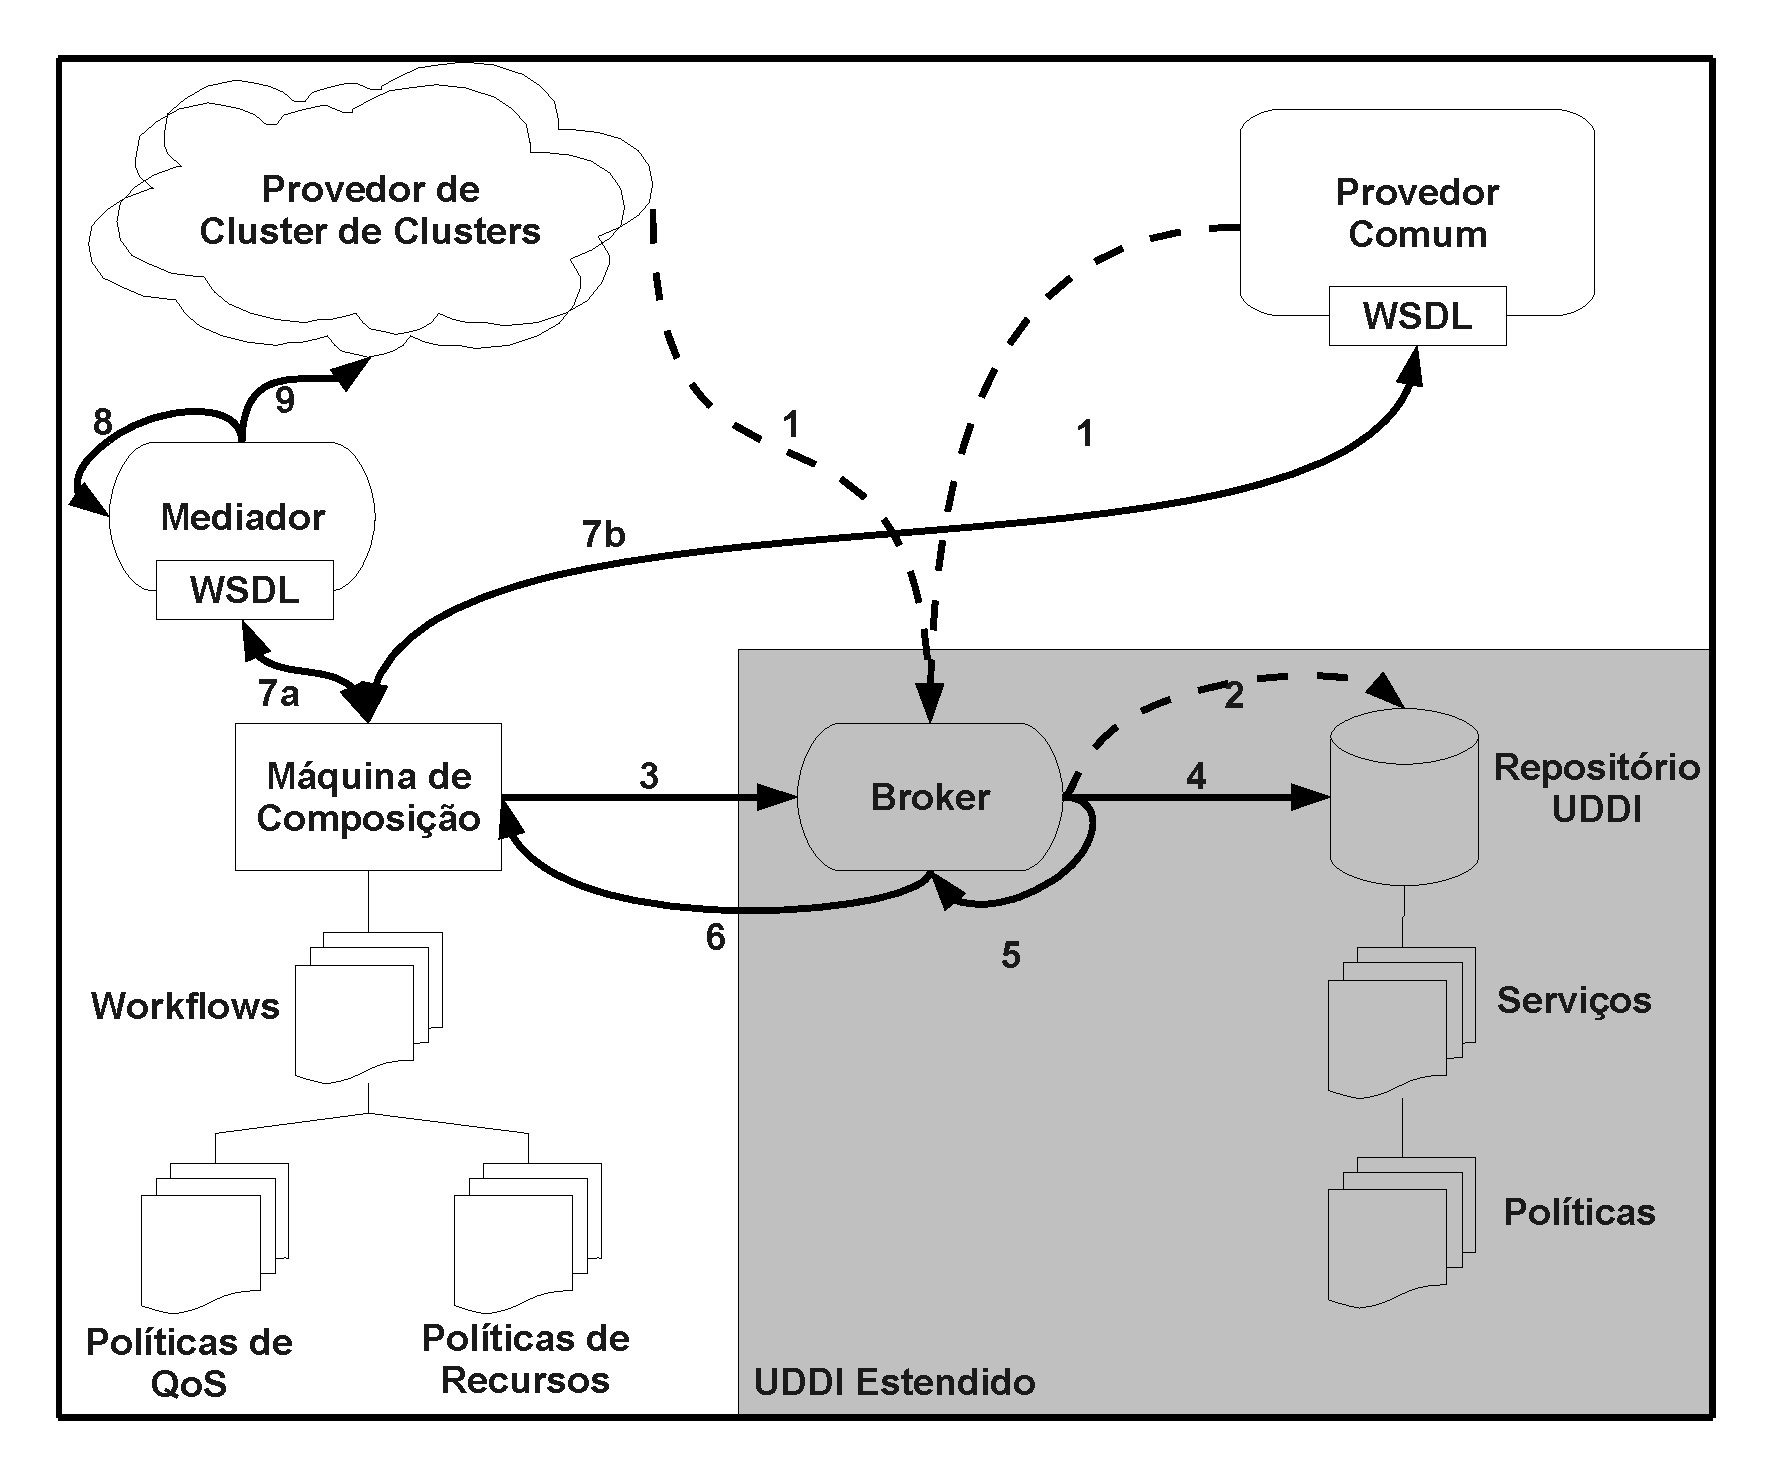
\includegraphics[scale=0.5]{imagens/execComposicaoG.pdf} 
		\caption[Arquitetura proposta para execução de \textit{workflows} descritos em WS-BPEL que podem utilizar recursos de um CoC.]{Arquitetura proposta para execução de \textit{workflows} descritos em WS-BPEL que podem utilizar recursos de um CoC. Componentes em branco foram desenvolvidos nesta dissertação e componentes em cinza foram propostos por Garcia e Toledo~\cite{DiegoUDDI}.}
		\label{fig:ArqComposicaoGen}
	    \end{center}
	\end{figure}
    
	O \texttt{Broker} é responsável por publicar as descrições dos serviços no \texttt{Repositório UDDI}.    
	Assim, os provedores de serviço precisam enviar suas políticas de QoS de seus serviços para o \texttt{Broker}, junto com a informação funcional tipicamente armazenada em um registro UDDI.
	Durante a execução, a \texttt{Máquina de Composição} é configurada com uma composição em WS-BPEL.
	Em sequida, quando o \textit{workflow} é iniciado e um serviço precisa ser executado, a \texttt{Máquina de Composição} envia ao \texttt{Broker} um pedido de seleção de implementação.
	A requisição inclui requisitos funcionais, que indicam o tipo de implementação necessária, e politicas de QoS e de recursos associadas ao serviço, indicando os requisitos do usuário, como, por exemplo, poder de processamento necessário (política de recurso) e tempo limite de resposta (política de QoS).

	Portanto, para cada serviço no \textit{workflow}, o \texttt{Broker} seleciona  uma implementação entre os serviços publicados no \texttt{Repositório UDDI}.
	Esta seleção compreende três fases;
	na primeira, o \texttt{Broker} seleciona serviços com as funcionalidades necessárias no UDDI, utilizando o mecanismo de busca do mesmo.
	Um conjunto de serviços é retornado ao \texttt{Broker}.
	Em seguida, as políticas dos consumidores e fornecedores são combinadas, permitindo ao \texttt{Broker} selecionar serviços adequados.
	Finalmente, o \texttt{Broker} envia os endereços de serviços para a \texttt{Máquina de Composição}, que invoca a tarefa.
	Se o serviço deve ser executado no CoC, a tarefa é enviada ao \texttt{Mediador}, que se encarrega de verificar os recursos necessários, submeter a tarefa, e a monitorar.
	Caso contrário, um \texttt{Provedor Comum} é invocado.	

	Em tempo de especificação, provedor e consumidor devem:
	\begin{enumerate}
	    \item O provedor faz uma requisição para a publicação de um serviço, especificando a descrição funcional (WSDL) e as políticas (WS-Policy) (Passo~1 na \autoref{fig:ArqComposicaoGen}), essa informação é passada para o \texttt{Repositório UDDI};
	    \item O consumidor especifica sua composição suas políticas para cada serviço.
	\end{enumerate}

	Em tempo de execução:
	\begin{enumerate}
	    \item Quando uma chamada de serviço é alcançada, a \texttt{Máquina de Composição} requisita uma seleção de implementação provendo requisitos funcionais e políticas ao \texttt{Broker} (Passo~3 na \autoref{fig:ArqComposicaoGen}); 
	    \item O \texttt{Broker} busca serviços no \texttt{Repositório UDDI} de acordo com as funcionalidades necessárias (Passo~4) e faz o casamento das políticas dos consumidores com a dos fornecedores (Passo~5);
	    \item O \texttt{Broker} informa os serviços selecionados à \texttt{Máquina de Composição} (Passo~6);
	    \item Para serviços que devem ser executados em um \texttt{Provedor de CoC}, a \texttt{Máquina de Composição} o executa usando o \texttt{Mediador} (Passo~7a);
	    \item O \texttt{Mediador} funciona como um \textit{proxy}, seleciona os recursos do CoC de acordo com os requisitos definidos nas políticas (Passo~8), envia o serviço a ser executado (Passo~9), o monitora e envia a resposta de volta para a \texttt{Máquina de Composição};
	    \item Para serviços comuns, a \texttt{Máquina de Composição} invoca a operação no serviço selecionado através do ponto de acesso do \texttt{Provedor Comum} retornado (Passo~7b).	   
	\end{enumerate}	

	A abordagem sugerida permite que novas aplicações, desenvolvidas como composições WS-BPEL, executem em conjunto a aplicações antigas, sem requerer nenhum tipo de modificação.
	Um estudo de caso com exemplo de de aplicação dessa arquitetura será mostrado em seguida.

    \section{Estudo de caso: SHARCNET}
    \label{sec:EstudoDeCasoSHARCNET}
	Para avaliar a arquitetura proposta era necessário implementá-la em um \textit{Multi-Clusters} real, para isso foi escolhida a rede SHARCNET.

	\subsection{SHARCNET}
	\label{subsec:SHARCNET}
	    Estruturada em forma de um \textit{Cluster} de \textit{Clusters}, a SHARCNET é uma rede multi-institucional de \textit{clusters} de alta performance distribuídos em dezesseis instituições acadêmicas na província de Ontário, no Canadá~\cite{Bauer07}.
	    Atualmente, esse sistema abriga pesquisas tanto das diversas áreas que tradicionalmente necessitam de computação de alta performance, como química, física, ciência dos materiais e engenharia, quanto estudos de outras áreas, incluindo negócios, economia e biologia.
	    
	    Essa rede tem três \textit{clusters} primários que já foram listados no \textit{Top 500}~\cite{top500:website} de supercomputadores.
	    Respectivamente, esses três \textit{clusters} contêm 267 nós com 1068 processadores, 768 nós com 1536 processadores e 768 nós com 3072 processadores;
	    cada um deles provê 70TB de armazenamento de alta velocidade.
	    Além disso, também existem outros 17 \textit{clusters} secundários, variando de 32 a 64 nós e totalizando mais de 8.000 processadores e 200TB de armazenamento. 
	    A interconexão entre os nós em cada um inclui G2 Myrinet, Quadrics (Elan, Elan 4 e 3) e Gigabit Ethernet;
	    a comunicação entre eles é realizada através de uma rede dedicada de alta velocidade e de 10 Gibabit Ethernet.
	    Em conjunto, todos esses recursos criam uma ``grade computacional'', de alta performance~\cite{bauerHPC}.

	    Os sistemas operacionais são variantes do Linux.
	    O escalonamento de tarefas é realizado pelo Load Sharing Facility (LSF) e a computação paralela pode ser implementada utilizando MPI ou OpenMPI.
	    As contas são gerenciadas pelo Lightweight Directory Access Protocol (LDAP), que permite que os pesquisadores utilizem apenas uma conta para acessar qualquer um dos \textit{clusters}~\cite{bauerHPC}.

	    Os \textit{clusters} da rede estão situados a uma distância considerável uns dos outros e são conectados por uma rede dedicada de fibra ótica.
	    Cada um deles tem um nó central que atua como escalonador local; entretanto, não existe um escalonador global, capaz de escalonar tarefas entre \textit{clusters} distintos.
	    Portanto, cada usuário deve manualmente verificar a carga atual e a capacidade de cada um, e escolher o que atende melhor os seus requisitos~\cite{Chau03}.

	    Assim, o balanceamento e a seleção de recursos não é transparente, como deveria ser em uma grade computacional.
	    Assim, a SHARCNET não é capaz de executar tarefas de maneira automática, como no caso de um sistema de gerência de workflows.	     
	    Consequentemente, os usuários acabam focando nos mesmo recursos, sobrecarregado um único \textit{cluster}, mesmo que existam outros com uma carga menor.
	    Além do mais, os usuários são obrigados a modificar manualmente a submissão de tarefas quando o \textit{cluster} que está sendo utilizado tem algum tipo de problema.

	    Por esse motivo, este trabalho propõe um escalonador global para a SHARCNET, permitindo a submissão automática de tarefas e a execução de \textit{workflows}. 

	    Como discutido anteriormente, a seleção de \textit{clusters} será baseada em requisitos de QoS e de recursos especificados na composição descrita pelo WS-BPEL estendido, também proposto neste trabalho.
	    Essa abordagem não requer modificações na estrutura do sistema, portanto mantém a compatibilidade com a seleção manual de recursos utilizada até então e permite que aplicações existentes se mantenham inalteradas.	    
	    
	    O escalonador global é discutido na \autoref{subsec:EscalonadorGlobal} e a arquitetura implementada para a execução de \textit{workflows} na SHARCNET é apresentada na \autoref{subsec:ArquiteturaAplicada}.     	

	\subsection{Arquitetura Aplicada}	
	\label{subsec:ArquiteturaAplicada}
	    A \autoref{fig:ArqComposicaoA} retrata a arquitetura aplicada para a execução de \textit{workflows} que podem utilizar recursos da SHARCNET.
	    Alguns novos elementos tiveram que ser incluídos para atender requisitos específicos desse ambiente.
	    Primeiramente, a \texttt{Máquina de Composição} foi alterada para invocar as tarefas e receber a resposta correspondente através de uma \texttt{Interface de Callback}.
	    Segundo, o \texttt{Escalonador Global}, explicado na \autoref{subsec:EscalonadorGlobal}, foi adicionado ao \texttt{Mediador}.
	    Finalmente, o \texttt{Monitor} foi adicionado, com a responsabilidade de monitorar as tarefas em execução na SHARCNET e, quando estas estiverem completas, enviar os resultados para a \texttt{Máquina de Composição}.
	    
	    \begin{figure}[!htb]%Figura:Arquitetura implementada
	    \begin{center}
		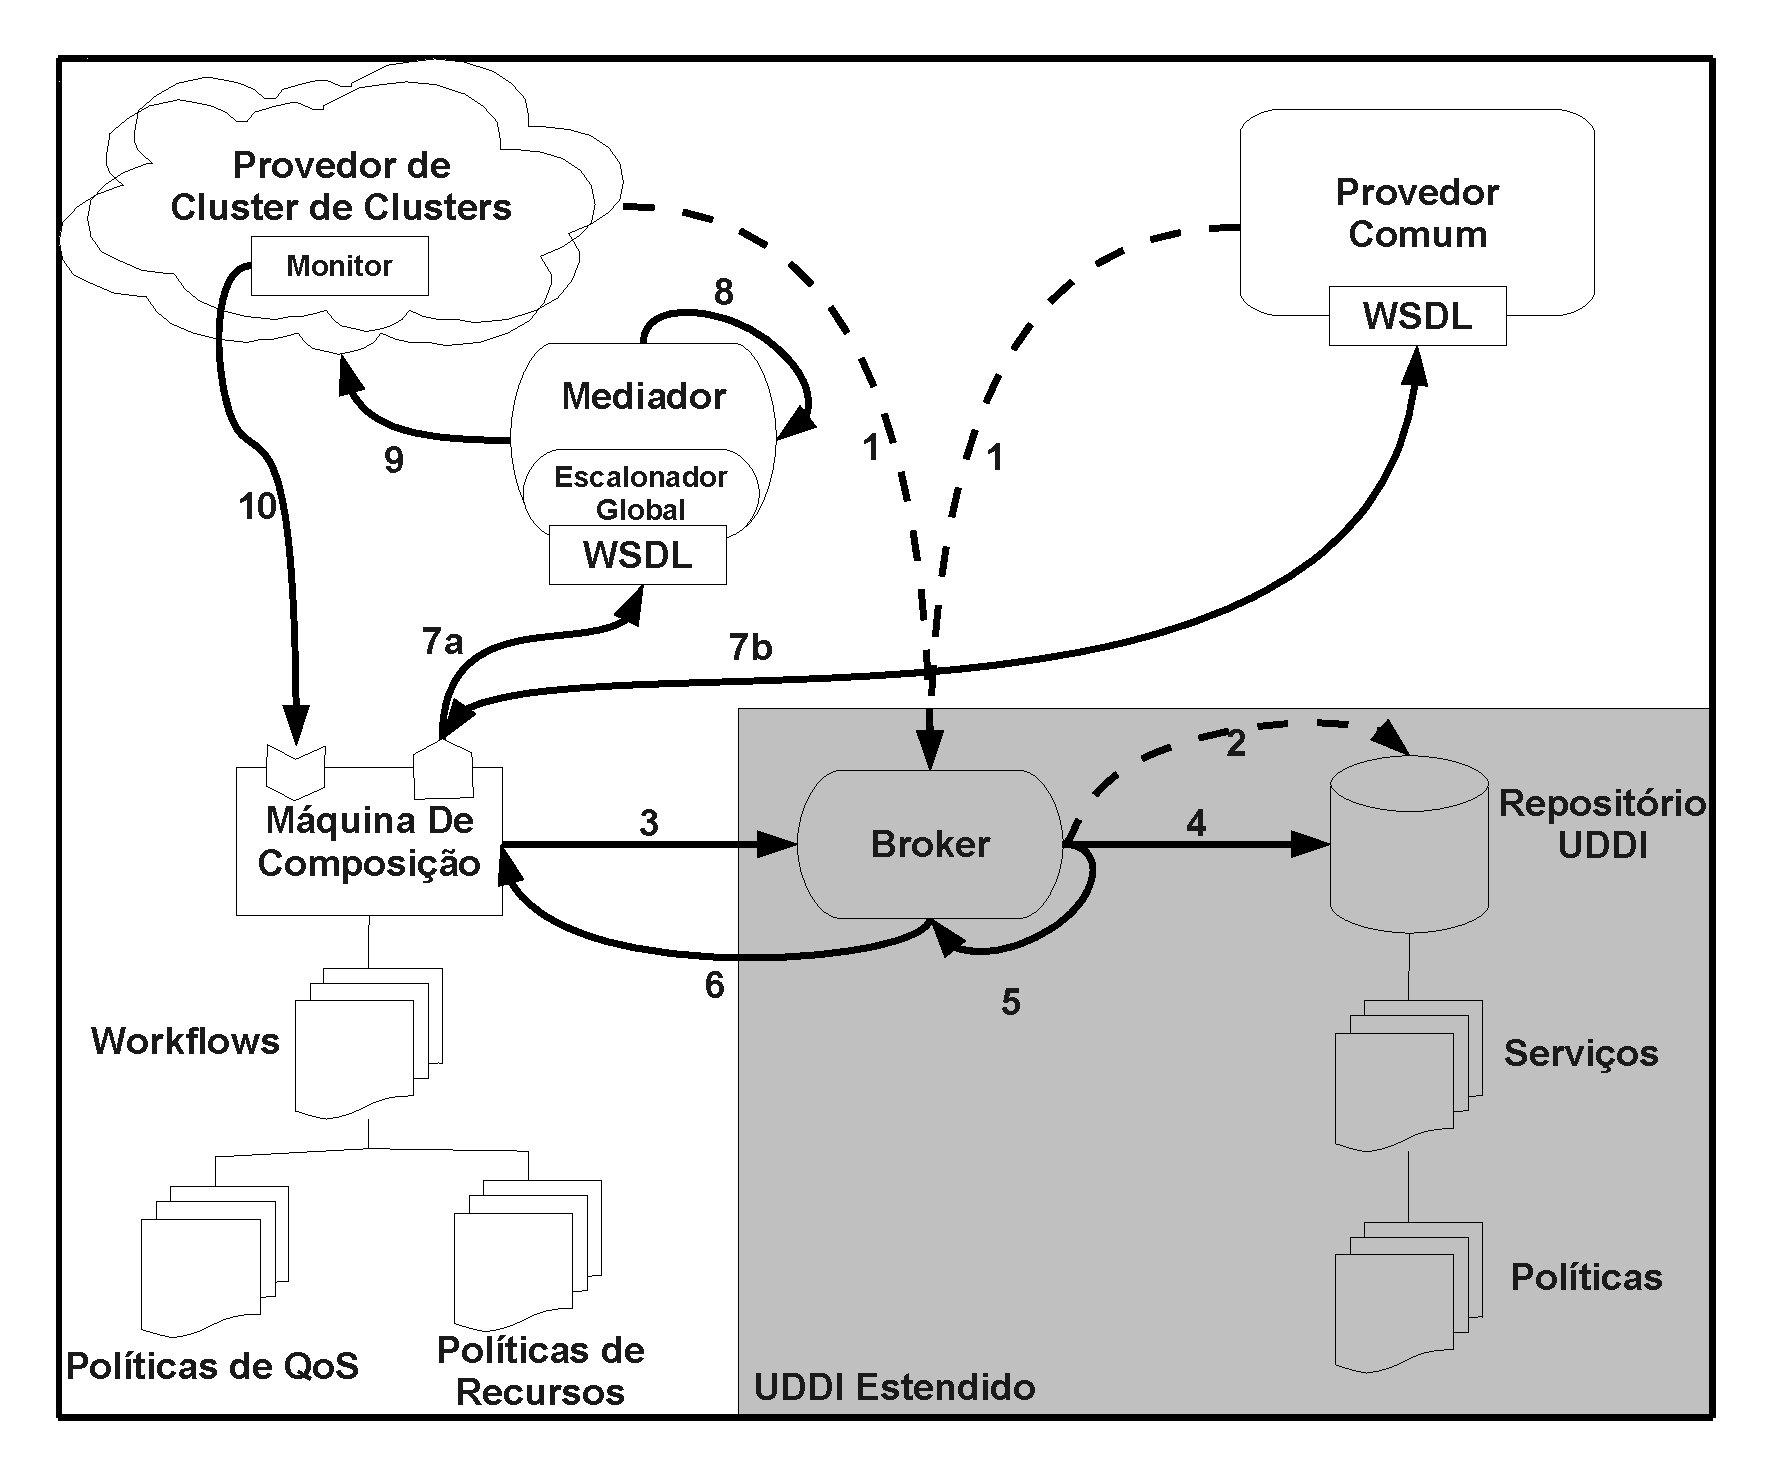
\includegraphics[scale=0.40]{imagens/execComposicaoA.pdf} 
		\caption{Arquitetura implementada.}
		\label{fig:ArqComposicaoA}
	    \end{center}
	    \end{figure}
	    
	    O usuário inicia uma execução de \textit{workflow}.
	    A \texttt{Máquina de Composição} invoca o \texttt{Broker} buscando serviços que atendam as especificações funcionais e de QoS. 
	    A \texttt{Máquina de Composição} invoca o \texttt{Mediador} como um serviço Web assíncrono, informando os requisitos de recursos utilizando o WS-PolicyAttachment em conjunto com o WS-Policy e a \texttt{Interface de Callback} utilizando o  WS-Addressing.
	    O \texttt{Mediador} atua como um \textit{proxy}, seleciona o \textit{cluster} mais adequado utilizando o \texttt{Escalonador Global}, e submete a tarefa.
	    Em seguida, o serviço \texttt{Monitor} é criado para monitorar a tarefa até que ela esteja completa.
	    Então, o resultado é enviado ao endereço de \textit{callback} especificado com o WS-Addressing, a tarefa é considerada completa e o \textit{workflow} continua a execução.	    	    

	    A arquitetura implementada permite a execução de \textit{workflows} utilizando recursos da SHARCNET de maneira automática e transparente.
	    Os detalhes de cada componente da arquitetura são explicados em seguida.	    	        
        

	\subsubsection{Máquina de Composição}
	O componente mais importante para a execução de um processo BPEL é a \texttt{Máquina de Composição}.
	A utilizada neste trabalho foi a \textit{BPEL Service Engine}, um \textit{plugin} para a execução de \textit{wokflows} no pacote Glasfish Open ESB do Netbeans~\cite{ESB:website}.
	Toda a arquitetura foi adaptada para utilizar as funcionalidades providas por padrão por esse componente, portanto não foi necessário modificá-lo.	
	
	\subsubsection{Broker}
	\label{subsec:Broker}
	Parte principal do UDDI estendido proposto por Garcia e Toledo~\cite{DiegoUDDI}.
	Este componente funciona como um WS fazendo uma interface para o repositório UDDI.
	Ao invés do usuário (\texttt{Máquina de Execução}) fazer uma busca por serviços utilizando o UDDI diretamente, ele utiliza o \texttt{Broker}, que faz as buscas baseadas em requisitos funcionais e de QoS.
	Como retorno, o \texttt{Broker} envia o endereço do serviço mais indicado.
		
	Essa etapa de busca deve ser adicionada explicitamente pelo usuário na composição BPEL.
	Em seguida a \texttt{Máquina de Composição} deve ser configurada para, em tempo de execução, utilizar o endereço recebido como resposta do \texttt{Broker} para o serviço a ser executado em seguida.
	Essa técnica é conhecida como \textit{Binding} Dinâmico.
	
	A \autoref{fig:BindingDinamico} retrata esta funcionalidade no Netbeans.
	O parâmetro \texttt{return}, da variável que recebe a saída do \texttt{Broker}, é atribuído ao parâmetro URL, das propriedades SOAP do serviço \texttt{ExecSharcnetIn}.
	O \autoref{cod:CodBindingDinamico} mostra o trecho de código BPEL associado a esta operação.
	
	\begin{figure}[!htb]%Figura:Binding Dinamico
	    \begin{center}
		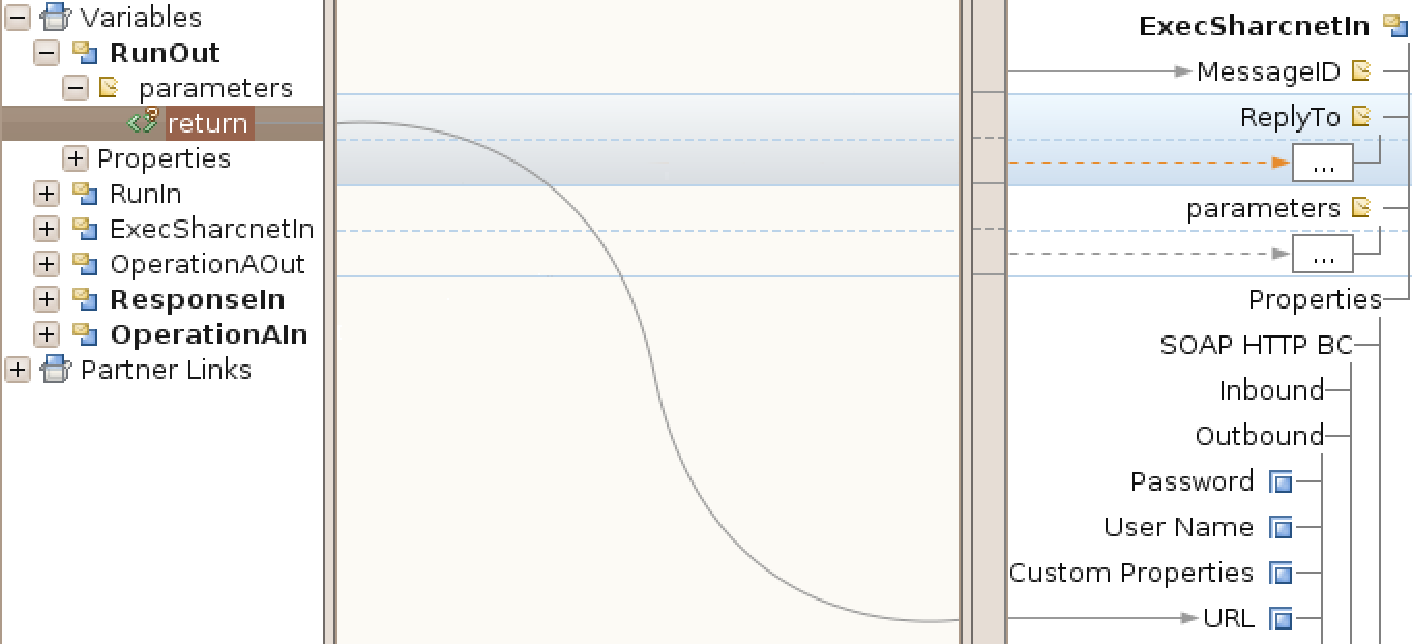
\includegraphics[scale=0.65]{imagens/BindingDinamico.pdf} 
		\caption{Configurando um \textit{binding} dinâmico no Netbeans.}
		\label{fig:BindingDinamico}
	    \end{center}
	\end{figure}
	
	%Codigo Binding Dinamico
% 	\begin{figure}[!htb]
% 	    \centering
 	    \lstinputlisting[float=!htb,language=XML,
			    caption={Trecho de código demonstrando um \textit{Binding} Dinâmico.},
			    label=cod:CodBindingDinamico]{listings/bindingDinamico.xml}
% 	    \caption{Trecho de código demonstrando um \textit{Binding} Dinâmico.}
% 	    \label{fig:CodBindingDinamico}
% 	\end{figure}
	    
	\subsubsection{UDDI}
	O repositório UDDI utilizado pelo \texttt{Broker} é o JUDDI~\cite{JUDDI:website}.
	O funcionamento detalhado desse componente da arquitetura é descrito na \autoref{subsec:UDDI}.
	
	Aqui, seu papel é armazenar os serviços publicados e auxiliar o \texttt{Broker} nas buscas por serviços.
		
	\subsubsection{Mediador}
	\label{subsec:Mediador}
	O \texttt{Mediador} é um elemento importante da arquitetura.
	Se trata de um WS desenvolvido em Java que atua como um \textit{proxy}, fazendo a interface entre a \texttt{Máquina de Composição} e a SHARCNET.
	Todas as requisições direcionadas a ela devem ser enviadas ao \texttt{Mediador}.
	Ele é responsável por gerenciar a execução das tarefas.
	Verifica os requisitos descritos pelo usuário em suas políticas e, utilizando outros componentes da arquitetura, encontra o melhor \textit{cluster} para executar a tarefa e monitora a sua execução.
	
	Esse componente, como a maior parte da estrutura, não é centralizado.
	Portanto, cada cliente pode ter um \texttt{Mediador} rodando localmente, mantendo a característica distribuída do sistema.
	
	Inicialmente o serviço deve ser configurado com os \textit{clusters} da SHARCNET.
	Essa configuração é feita através do arquivo \textit{config.ini} retratado no \autoref{cod:configClusters}.	
	
	%Configuracao de clusters
% 	\begin{figure}[!htb]
% 	    \centering
 	    \lstinputlisting[float=!htb,language=XML,
			    caption={Configurações de servidores no arquivo \texttt{config.ini}.},
			    label=cod:configClusters]{listings/config.ini}
% 	    \caption{Configurações de servidores no arquivo \texttt{config.ini}.}
% 	    \label{fig:configClusters}
% 	\end{figure}
	
	Para executar esse serviço, o usuário deve invocá-lo na composição BPEL de forma assíncrona.
	Essa operação é composta de três etapas.
	Primeiramente o usuário deve invocar o \texttt{Mediador} através da função \texttt{INVOKE} do BPEL usando a interface WSDL demonstrada, de forma simplificada e apenas com seus componentes mais importantes, no \autoref{cod:wsdlMediadorInvoke}.
	Nas linhas de 3 a 7 vemos a construção da mensagem dividida em três partes: O \texttt{MessageID}, parte da descrição WS-Addressing que define um código único para a mensagem; o \texttt{ReplyTo}, parte da descrição WS-Addressing que define o endereço da interface de \textit{callback} que deve receber a resposta e; o \texttt{parameters}, outros parâmetros necessários para executar o serviço.
	As linhas de 13 a 17 informam que o \texttt{MessageID} e o \texttt{ReplyTo} fazem parte co cabeçalho e o \texttt{parameters} faz parte do corpo da mensagem.
	
	%WSDL Invoke Mediador
% 	\begin{figure}[!htb]
% 	    \centering
 	    \lstinputlisting[float=!htb,language=XML,
			    caption={Componentes principais da interface WSDL para invocar o \texttt{Mediador}.},
			    label=cod:wsdlMediadorInvoke]{listings/wsdlMediadorInvoke.xml}
% 	    \caption{Componentes principais da interface WSDL para invocar o \texttt{Mediador}.}
% 	    \label{fig:wsdlMediadorInvoke}
% 	\end{figure}

	O \autoref{cod:xsdMediadorInvoke} retrata o esquema XML que detalha os tipos de dados do elemento \texttt{execSharcnet}, tipo do atributo \texttt{parameters}.
	Os seguintes elementos são identificados:
	
	\begin{itemize}
	 \item \textbf{server}: Parâmetro que define o \textit{cluster} que deve executar a tarefa. Geralmente é utilizado o valor \texttt{AUTO}, que informa que o \texttt{Escalonador Global} deve automaticamente escolher o melhor \textit{cluster}. Caso outro valor seja informado o \texttt{Escalonador Global} não é executado e o \textit{cluster} especificado é executado diretamente;
	 \item \textbf{login}: Para executar qualquer função na SHARCNET é necessário possuir uma conta. Esse parâmetro é usado para informar o nome usuário do cliente;
	 \item \textbf{senha}: Senha do cliente de acesso à SHARCNET;
	 \item \textbf{servico}: Informa qual serviço deve ser executado na SHARCNET.	 
	\end{itemize}	
	
	%XSD Invoke Mediador
% 	\begin{figure}[!htb]
% 	    \centering
 	    \lstinputlisting[float=!htb,language=XML,
			    caption={Componentes principais do esquema XML do elemento \texttt{execSharcnet}.},
			    label=cod:xsdMediadorInvoke]{listings/xsdMediadorInvoke.xml}
% 	    \caption{Componentes principais do esquema XML do elemento \texttt{execSharcnet}.}
% 	    \label{fig:xsdMediadorInvoke}
% 	\end{figure}
		
	A segunda etapa para a execução do serviço de forma assíncrona consiste em ``implementar'' a interface de \textit{callback} para receber a resposta do serviço.
	Isso é feito através da função \texttt{RECEIVE} do BPEL.
	Essa interface é retratada no \autoref{cod:wsdlMediadorReply}.
	Nas linhas de 3 a 6 vemos a construção da mensagem dividida em duas partes: O \texttt{RelatesTo}, parte da descrição WS-Addressing que especifica qual mensagem originou a resposta e; o \texttt{parameters}, outros parâmetros necessários para executar o serviço.
	As linhas de 12 a 15 informam que o \texttt{RelatesTo} faz parte co cabeçalho e o \texttt{parameters} faz parte do corpo da mensagem.
	
	%WSDL Reply Mediador
% 	\begin{figure}[!htb]
% 	    \centering
 	    \lstinputlisting[float=!htb,language=XML,
			    caption={Componentes principais da interface WSDL de \textit{callback} do \texttt{Mediador}.},
			    label=cod:wsdlMediadorReply]{listings/wsdlMediadorReply.xml}
% 	    \caption{Componentes principais da interface WSDL de \textit{callback} do \texttt{Mediador}.}
% 	    \label{fig:wsdlMediadorReply}
% 	\end{figure}	
	
	O \autoref{cod:xsdMediadorReply} retrata o esquema XML que detalha os tipos de dados do elemento \texttt{response}, tipo do atributo \texttt{parameters}.
	Podemos identificar o elemento \texttt{result}, que é preenchido com a resposta do serviço executado na SHARCNET.		
	
	%XSD Reply Mediador
% 	\begin{figure}[!htb]
% 	    \centering
 	    \lstinputlisting[float=!htb,language=XML,
			    caption={Componentes principais do esquema XML do elemento \texttt{response}.},
			    label=cod:xsdMediadorReply]{listings/xsdMediadorReply.xml}
% 	    \caption{Componentes principais do esquema XML do elemento \texttt{response}.}
% 	    \label{fig:xsdMediadorReply}
% 	\end{figure}	
	
	Na terceira e última etapa, o usuário deve criar a correlação da mensagem de \texttt{INVOKE} com a de \texttt{RECEIVE}.
	Na \texttt{Máquina de Execução} podem existir diversos processos executando ao mesmo tempo.
	Por isso, ela precisa saber a que instância deve enviar uma resposta recebida na interface de \textit{callback}.
	Portanto, o usuário deve criar uma \texttt{Correlation} ligando o parâmetro \texttt{MessageID} da mensagem de \texttt{INVOKE} com o parâmetro \texttt{RelatesTo} da mensagem de \texttt{RECEIVE}.
	Essa ação está demonstrada na \autoref{fig:Correlation}.
	
	\begin{figure}[!htb]%Figura:Correlation
	    \begin{center}
		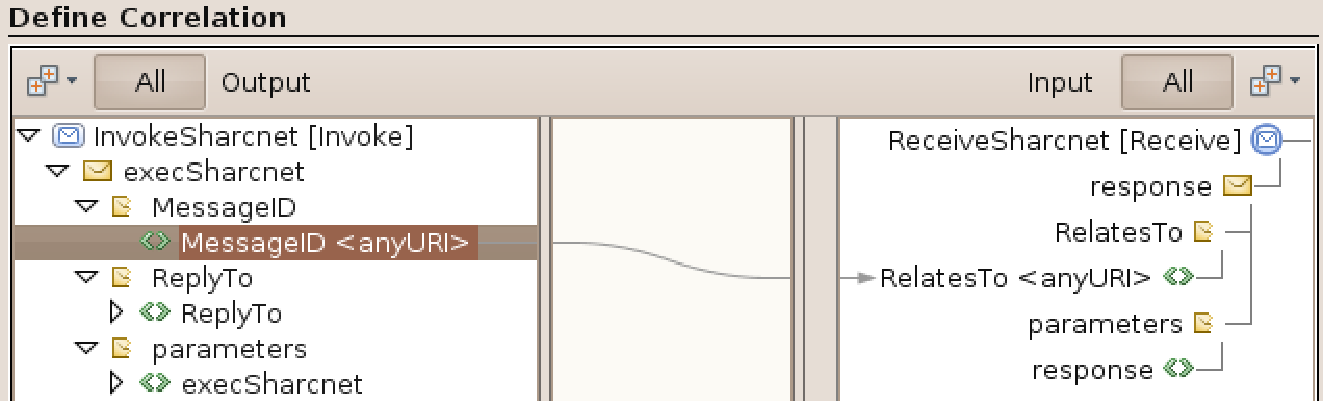
\includegraphics[scale=0.50]{imagens/Correlation.pdf} 
		\caption{Estrutura de \texttt{Correlation} sendo criada.}
		\label{fig:Correlation}
	    \end{center}
	\end{figure}
	
	\pagebreak %TODO: Coloquei pra ajustar a página... conferir se está OK.
	\subsubsection{Escalonador Global}
	\label{subsec:EscalonadorGlobal}
	    O \texttt{Escalonador Global}, ou Meta-Escalonador, é a parte da estrutura responsável por verificar o estado dos \textit{clusters} da SHARCNET e escolher o mais apropriado para enviar a tarefa.
	    Como ele foi planejado para ser implantado em um sistema com aplicações em execução, manter a compatibilidade com os métodos antigos de seleção de recursos se torna fundamental.
	    Entretanto, quando uma tarefa é submetida diretamente a algum \textit{cluster}, o novo escalonador não tem conhecimento.
	    
	    Esse cenário se assemelha ao funcionamento de pagamentos de contas em um banco, ilustrado na \autoref{fig:CenarioBanco}.
	    Por exemplo, um cliente pode saber em que agência (representando um \textit{cluster}) ele pode pagar a conta, quantas pessoas estão em cada fila (programas esperando para serem executados) e quantos funcionários estão atendendo (número de processadores disponíveis).
	    No entanto, ele não pode saber quanto tempo cada pessoa vai gastar no atendimento ou quantas pessoas vão estar na fila em algum momento no futuro.
	    
	    \begin{figure}[!htb]%Figura:Cenário de pagamento de contas em um banco
		\begin{center}
		    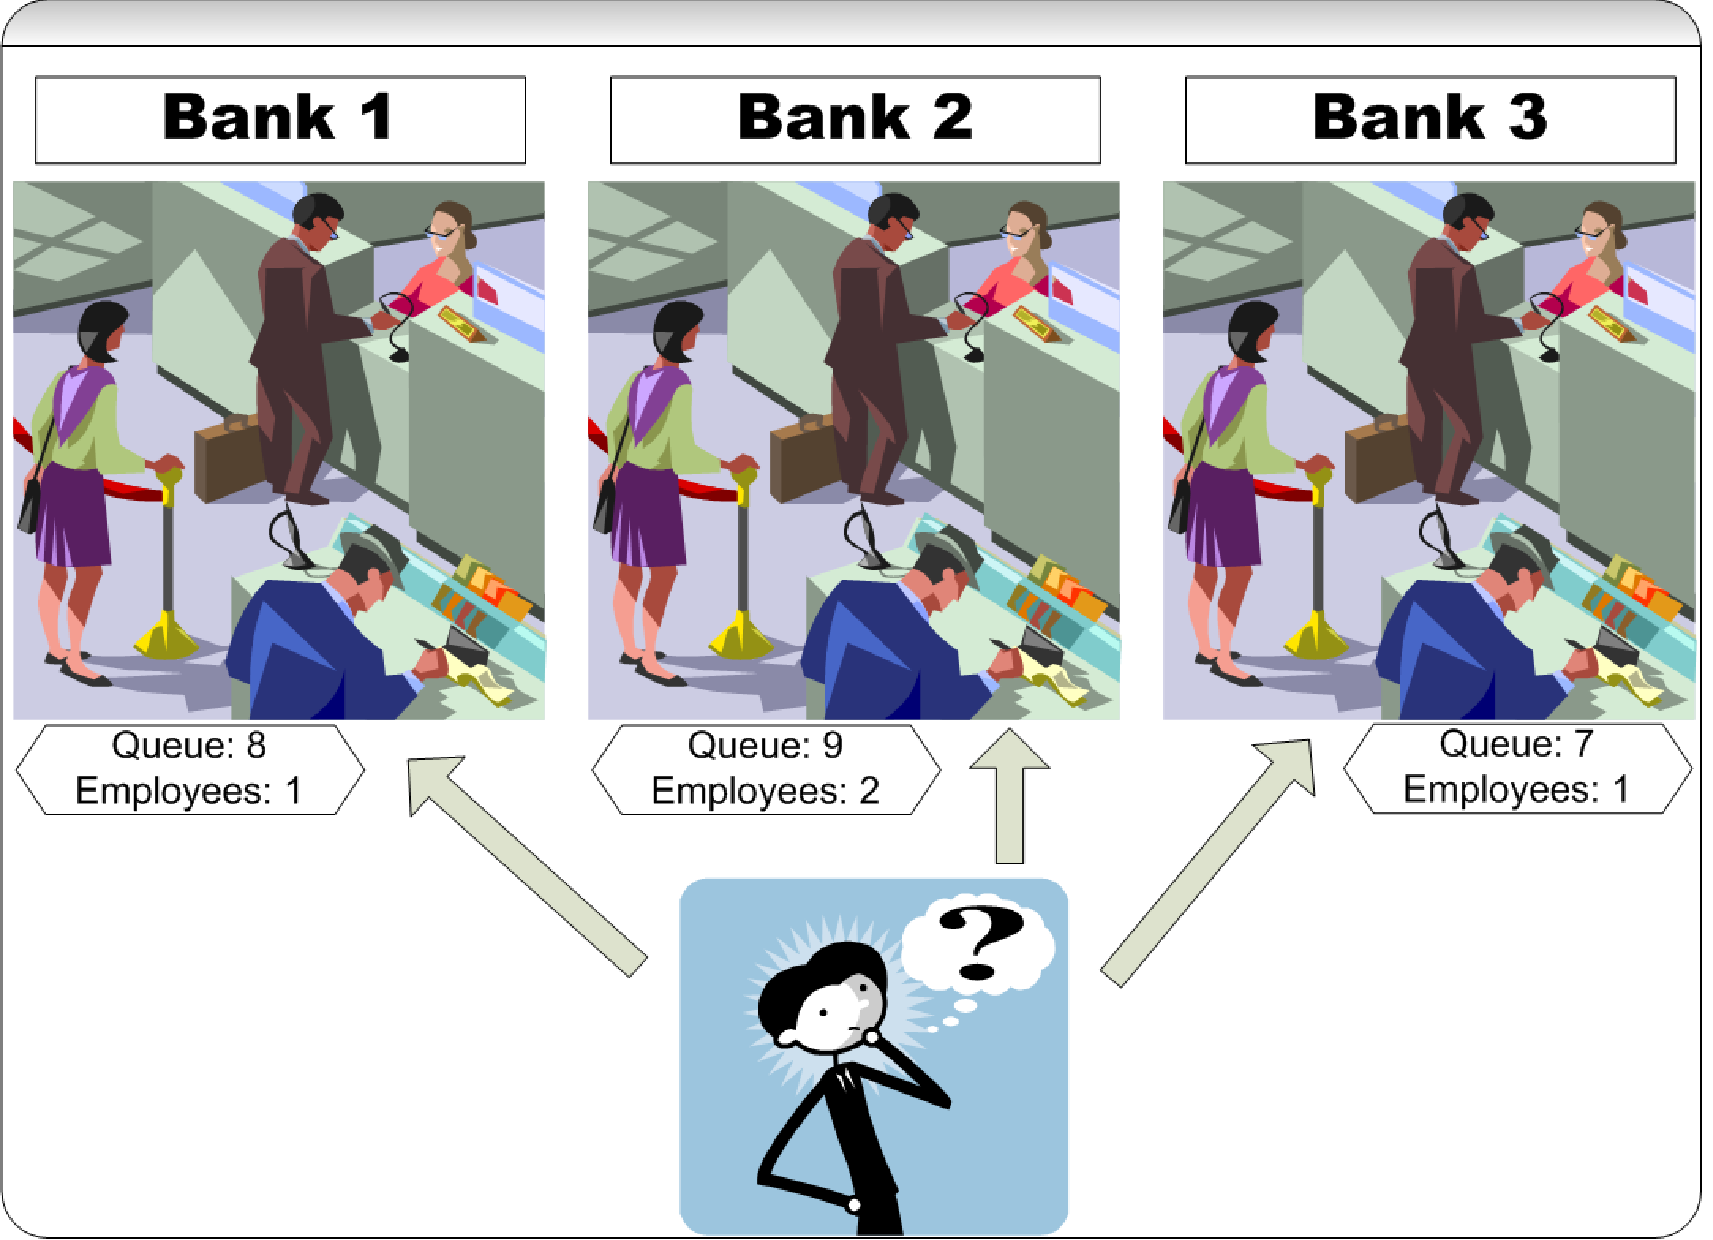
\includegraphics[scale=0.35]{imagens/banco.pdf}
		    \caption{Cenário de pagamento de contas em um banco.}
		    \label{fig:CenarioBanco}
		\end{center}
	    \end{figure}

	    O usuário envia os requisitos de sua tarefa em termos de memória, espaço em disco e quantidade de processadores.
	    Em seguida, o escalonador global seleciona um \textit{cluster} para executar a tarefa; o \textit{cluster} escolhido é o que tem a menor fila de espera entre os que atendem os requisitos do usuário.
	    Para comparar a carga de cada HPCC propomos a seguinte métrica, definindo o tamanho da fila pela seguinte \autoref{eq:fila}.

	    %Formula da fila
	    \begin{equation}
		\frac{Quantidade\; de\; processadores\; requisitados\; pela\; fila}{Quantidade\; total\; de\;  processadores * Potencia\; dos\; processadores}
		\label{eq:fila}
	    \end{equation}

	    Nessa fórmula, a quantidade total de processadores disponíveis no \textit{cluster} é multiplicada pelo seu poder de processamento, representando a capacidade total de um \textit{cluster}.
	    Então, o total de processadores requisitados pelos processos na fila é dividido por esse valor.
	    O número resultante representa a carga atual do \textit{cluster}.

	    Esse conceito foi implementado em uma aplicação desenvolvida na linguagem Python que se conecta a cada um dos \textit{clusters} cadastrados e busca o estado corrente do escalonador LSF local.
	    Utilizando os dados de cada um deles, o sistema seleciona o com a menor carga que atende aos requisitos do usuário e envia a tarefa, que agora passa a ser responsabilidade do escalonador local.
	    Para evitar sobrecarregar a rede com buscas desnecessárias, o software só verifica o estado dos \textit{clusters} quando existem tarefas para serem enviadas, além da possibilidade de configurar um tempo para armazenar as informações em \textit{cache}.
	    
	    O \autoref{cod:servers.conf} mostra um trecho do arquivo de configuração \texttt{servers.conf}, utilizado para armazenar as informações dos \textit{clusters} e configurar o tempo de \textit{cache}. A marcação \texttt{DEFAULT} guarda a informação de quando foi a última a atualização e o tempo que programa deve aguardar para se atualizar novamente. A marcação \texttt{requin} guarda as informações obtidas sobre o \textit{cluster} denominado \texttt{requin}, como endereço do servidor, quantidade de processadores, processos na fila, e outros.
	    
	    %Arquivo servers.conf
% 	    \begin{figure}[!htb]
% 		\centering
 		\lstinputlisting[float=!htb,language=XML,
				caption={Trecho do arquivo de configuração \texttt{servers.conf}.},
				label=cod:servers.conf]{listings/servers.conf}
% 		\caption{Trecho do arquivo de configuração \texttt{servers.conf}.}
% 		\label{fig:servers.conf}
% 	    \end{figure}

	    Esse método se mostra vantajoso de diversas maneiras.
	    Primeiramente, é simples e distribuído, permitindo que cada usuário execute o escalonador localmente, vendo a situação dos \textit{clusters}, e envie as tarefas ao mais apropriado de forma transparente.
	    Em segundo lugar, a abordagem não afeta a execução aplicações já existentes.
	    Finalmente, a única carga adicional é calcular a formula mostrada anteriormente.
	    A estrutura geral do \texttt{Escalonador Global} é descrita na \autoref{fig:SchedulerArchitecture}.
	    
	    \begin{figure}[!htb]%figura da arquitetura do escalonador
		\begin{center}
		    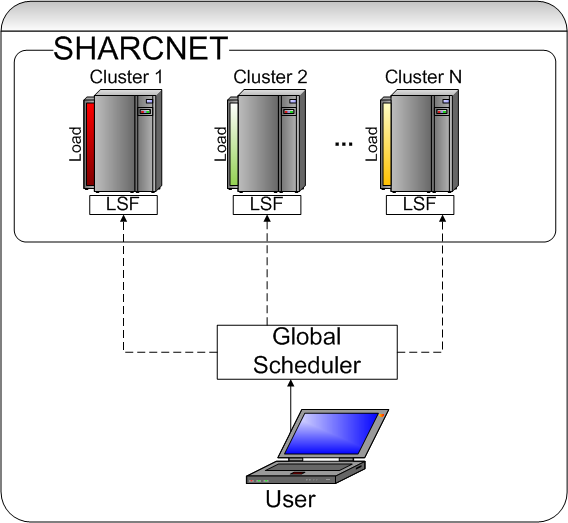
\includegraphics[scale=0.36]{imagens/scheduler.png} 
		    \caption{Arquitetura do Escalonador Global.}
		    \label{fig:SchedulerArchitecture}
		\end{center}
	    \end{figure}	 
	
	\subsubsection{Monitor}
	\label{subsec:Monitor}
	Aplicação desenvolvida na linguagem Python responsável por monitorar o estado dos serviços sendo executados na SHARCNET.
	Para cada tarefa que o \texttt{Mediador} envia para a SHARCNET, ele cria uma instância de \texttt{Monitor} para monitorá-la.
	O \texttt{Monitor} guarda o número de identificação da tarefa e utiliza funções do escalonador LSF local para verificar seu estado e aguardar a sua finalização.
	Quando a tarefa conclui sua execução, seu resultado é lido e enviado para o endereço de \textit{callback} especificado no WS-Addressing.
	
	\subsubsection{Provedor de CoC}
	O \texttt{Provedor de Cluster de Clusters} nada mais é do que a rede SHARCNET explicada na \autoref{subsec:SHARCNET}. Responsável por executar os serviços que necessitam de grande quantidade de poder computacional.
	
	\subsubsection{Provedor Comum}
	O \texttt{Provedor Comum} representa todos os provedores de serviços Web convencionais.
	
	Para demosntrar o funcionamento geral do sistema, as Figuras \ref{fig:imagemBPEL} e \ref{fig:DiagramaSequencia} exibem, respectivamente, diagrama BPEL necessário para a execução e a sequencia de ações tomadas para executar serviços que utilizam a SHARCNET.
		
	
	\begin{figure}[!htb]%Figura:Imagem BPEL
	    \begin{center}
		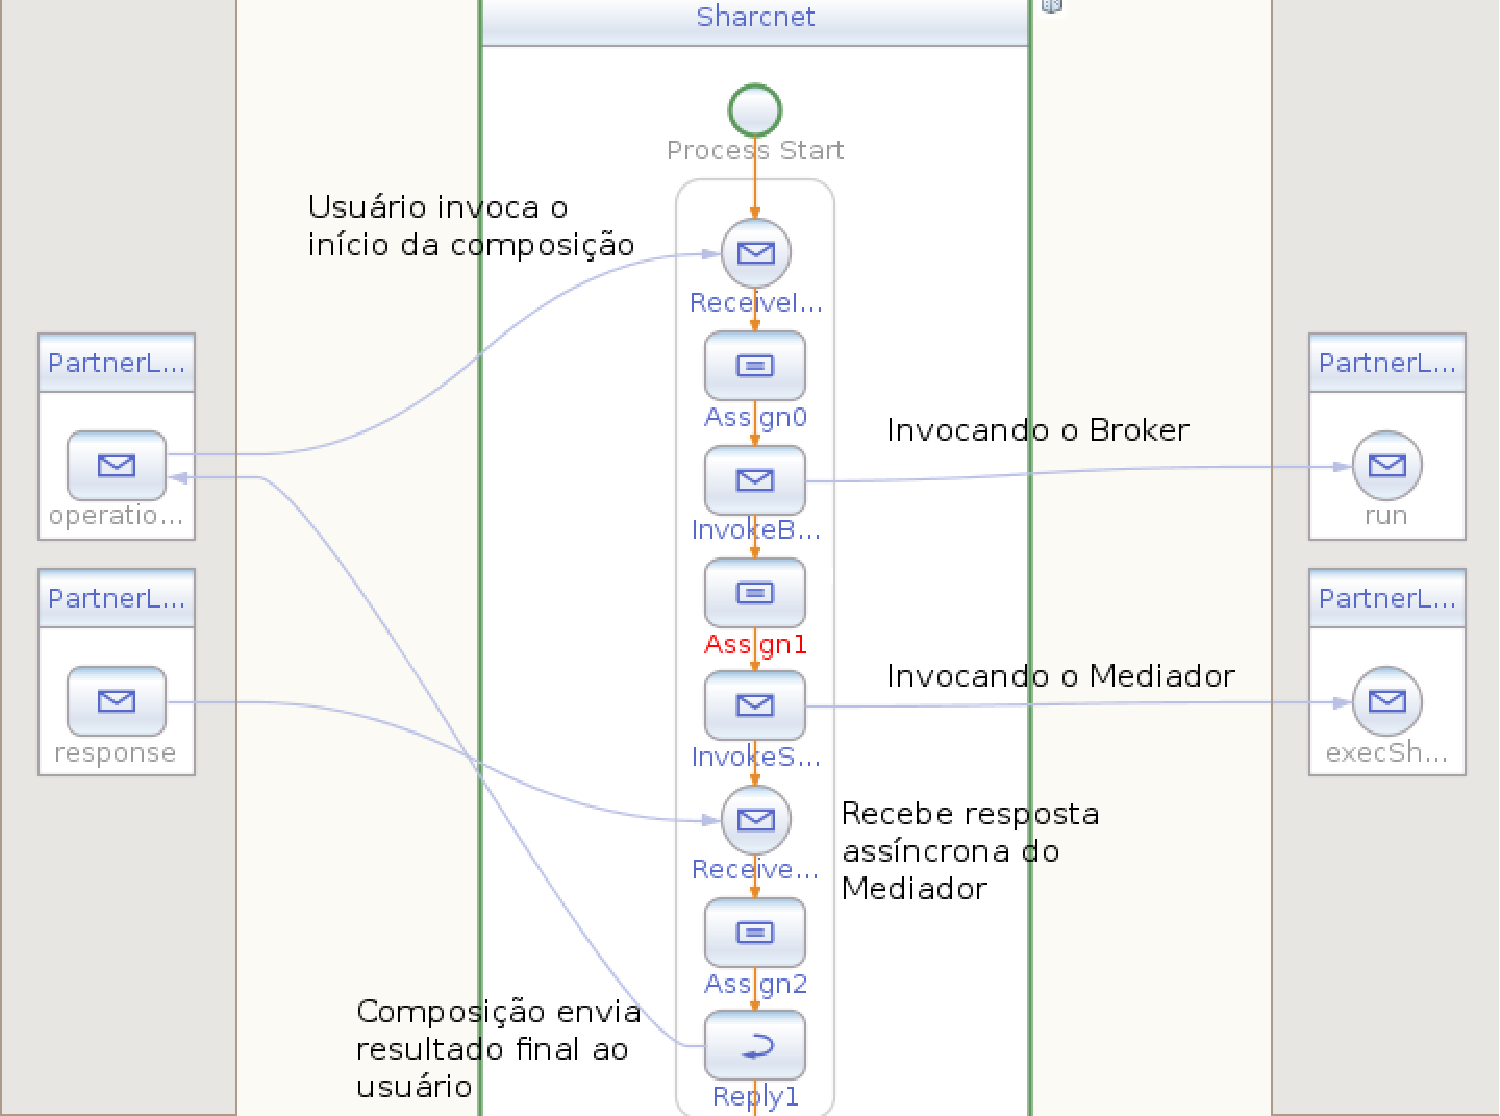
\includegraphics[scale=0.50]{imagens/imagemBPEL.pdf} 
		\caption{Diagrama BPEL mínimo para executar um serviço na SHARCNET.}
		\label{fig:imagemBPEL}
	    \end{center}
	\end{figure}  
	    
	\begin{figure}[!htb]%Figura:diagrama de sequencia
	    \begin{center}
		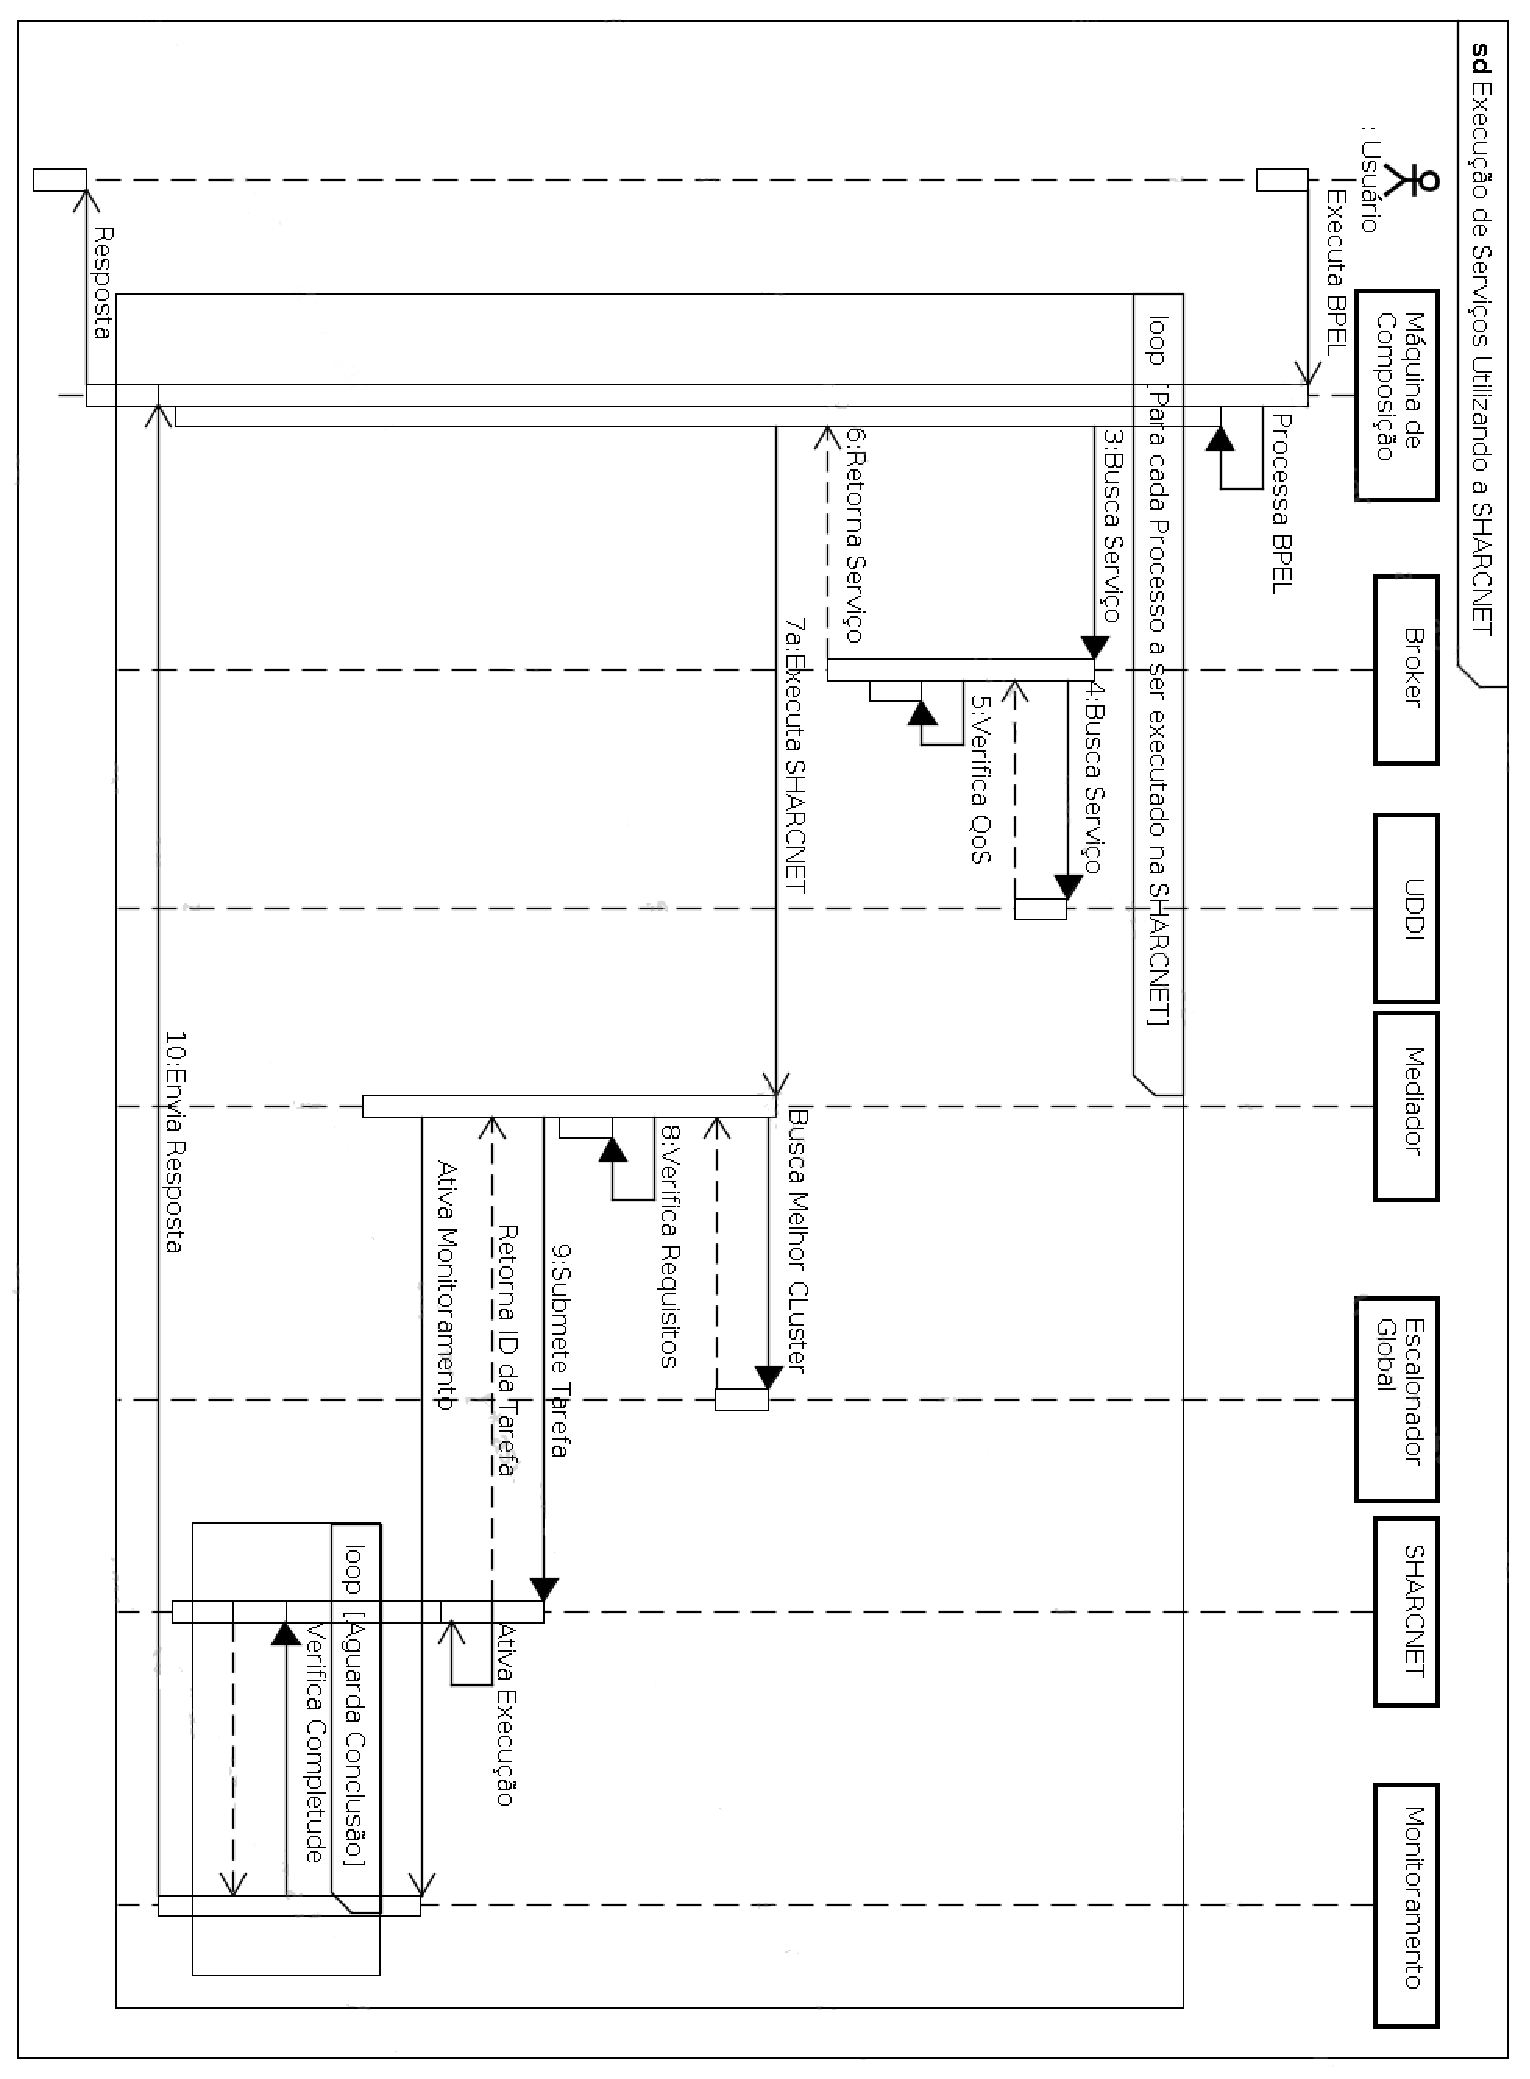
\includegraphics[scale=0.55]{imagens/sequencia.pdf} 
		\caption[Diagrama de sequência de uma execução de serviços utilizando a SHARCNET.]{Diagrama de sequência de uma execução de serviços utilizando a SHARCNET. Os números na imagem são referentes aos números na \autoref{fig:ArqComposicaoA}.}
		\label{fig:DiagramaSequencia}
	    \end{center}
	\end{figure}

\chapter{Aplicação}
\label{chap:Aplicacao}
    Para validar este trabalho e testar seu comportamento em um ambiente de produção, o mesmo foi aplicado em um problema real.
    Foi utilizado o \textit{workflow} de criação de mosaicos da aplicação Montage~\cite{Montage:website}, que junta diversas imagens para criar mosaicos personalizados do céu.
    Foram criados serviços que executam cada uma das etapas do algoritmo.
    As interações desses serviços foram especificadas em WS-BPEL e as partes mais custosas do algoritmo foram configuradas para serem executadas na rede SHARCNET.
    
    A \autoref{sec:Montage} explica com detalhes a aplicação Montage e seu \textit{workflow} para a criação de mosaicos.
    A \autoref{sec:ImplementacaoReal} demonstra os detalhes da implementação, como o processo BPEL, serviços e políticas.
    Por fim, a \autoref{sec:DiscussaoReal} discute as principais características, vantagens e desvantagens encontradas. 
    
    \section{Montage}
    \label{sec:Montage}
	O Montage~\cite{Montage:website} foi criado pela NASA como um conjunto de ferramentas de código aberto que pode ser usado para gerar mosaicos personalizados do céu através de imagens de entrada no formato FITS (Sistema de Transporte Imagem Flexível)~\footnote{Do inglês, \textit{Flexible Image Transport System}}.
	O algoritmo pode ser representado por um \textit{workflow} e é algumas vezes executado em ambientes de grade, como o TeraGrid~\cite{TeraGrid:website}.
	Durante a produção do mosaico, a geometria do produto final é calculada a partir da geometria das imagens de entrada.
	As entradas são então reprojetadas para ficarem na mesma escala espacial e rotação.
	As emissões de fundo das imagens são corrigidas para ficarem do mesmo nível em todas as imagens.
	As imagens reprojetadas e corrigidas são então unidas para formarem o mosaico final.
	%https://confluence.pegasus.isi.edu/display/pegasus/Montage+Characterization
	
	Neste trabalho foi utilizado um exemplo de criação de um mosaico a partir de 10 imagens do Atlas 2MASS da galáxia Pinwheel, ou M101.
	O \textit{workflow} é dividido em cinco etapas sequenciais e bem definidas: Reprojetar imagens, gerar mosaico inicial, modelar planos de fundo, combinar planos de fundo e gerar mosaico corrigido.
	
	A primeira etapa é a mais custosa de todo o \textit{workflow} e utiliza as ferramentas \texttt{mImgtbl} e \texttt{mProjExec} para, respectivamente, criar uma tabela de metadados descrevendo as imagens e reprojetá-las.
	Na segunda etapa as ferramentas \texttt{mAdd} e \texttt{mJPEG} são utilizadas para gerar o mosaico inicial, visto na \autoref{fig:Mosaico}.
	Em seguida, são utilizadas as ferramentas \texttt{mOverlaps}, \texttt{mDiffExec} e \texttt{mFitExec} para suavizar os níveis de fundo entre as imagens sobrepostas.
	Após, os ajustes de plano de fundo são combinados e aplicados na imagem original reprojetada usando as ferramentas  \texttt{mBgModel} e \texttt{mBgExec}.
	Por fim, o mosaico corrigido é gerado. Para isso as ferramentas \texttt{mAdd} e \texttt{mJPEG} são utilizadas novamente.
	A \autoref{fig:MosaicoCorrigido} mostra o mosaico final corrigido.
	%Descrição Tutorial: http://irsa.ipac.caltech.edu/Montage/docs/m101tutorial.html
	%-----
	%Algoritmos: http://irsa.ipac.caltech.edu/Montage/docs/algorithms.html#coadd
	
	
	\begin{figure}[!htb]%Imagens geradas da M101
	    \begin{minipage}[b]{0.5\linewidth} % A minipage that covers half the page
		\centering
		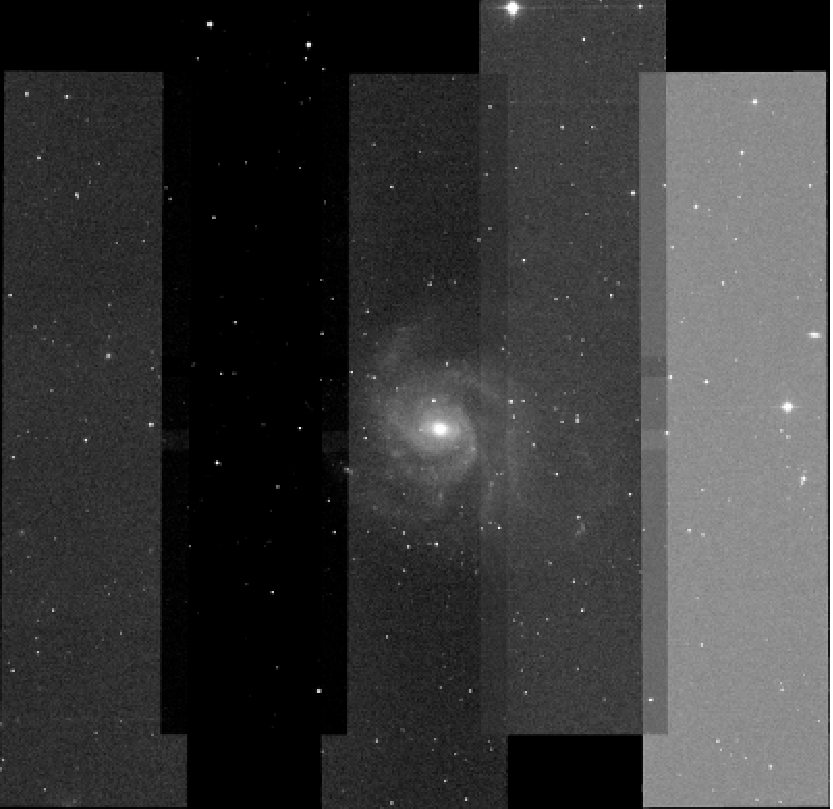
\includegraphics[scale=0.5]{imagens/mosaico1.pdf} 
		\caption{Mosaico M101 não corrigido.}
		\label{fig:Mosaico}
	    \end{minipage}
	    \hspace{0.2cm} % To get a little bit of space between the figures
	    \begin{minipage}[b]{0.5\linewidth}
		\centering
		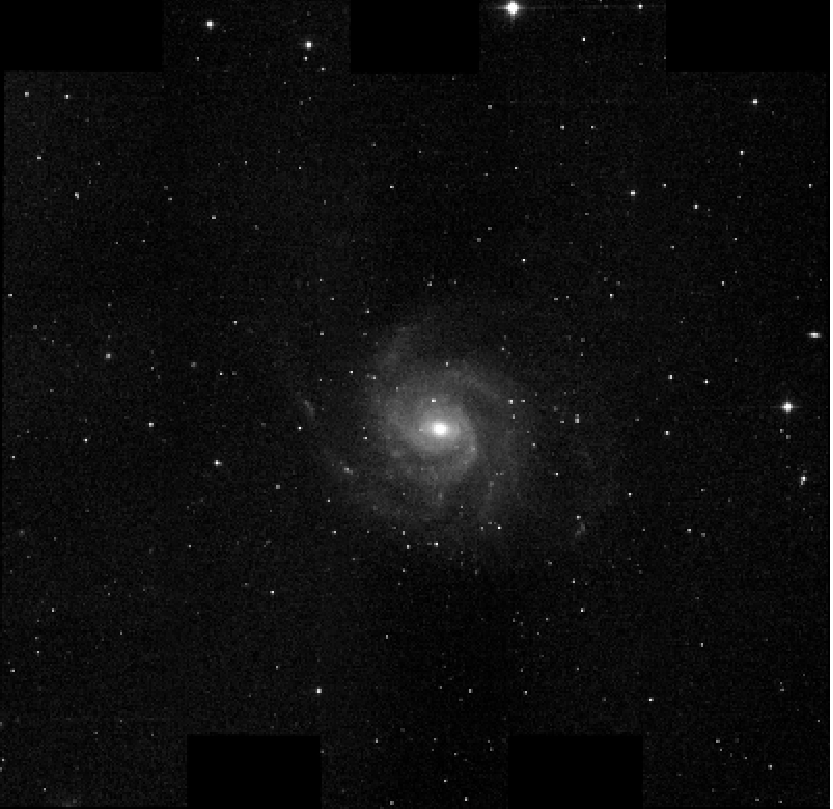
\includegraphics[scale=0.5]{imagens/mosaico2.pdf} 
		\caption{Mosaico M101 corrigido.}
		\label{fig:MosaicoCorrigido}
	    \end{minipage}
	\end{figure}	    
	    
% 	\begin{figure}[!htb]%Figura:Mosaico M101 não corrigido
% 	    \begin{center}
% 		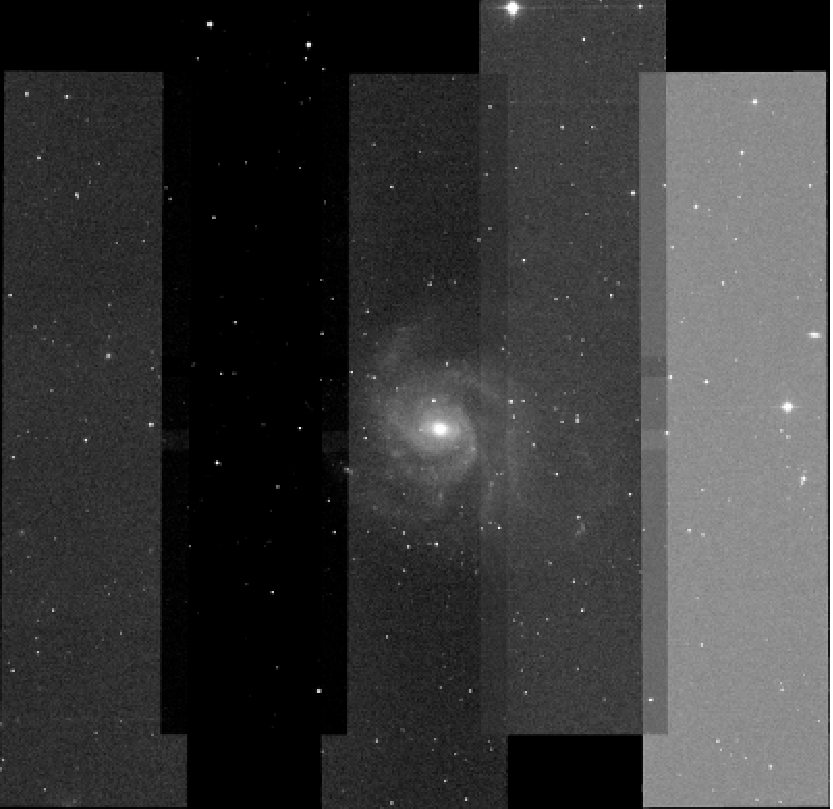
\includegraphics[scale=0.5]{imagens/mosaico1.pdf} 
% 		\caption{Mosaico M101 não corrigido.}
% 		\label{fig:Mosaico}
% 	    \end{center}
% 	\end{figure}
    
% 	\begin{figure}[!htb]%Figura:Mosaico M101 corrigido
% 	    \begin{center}
% 		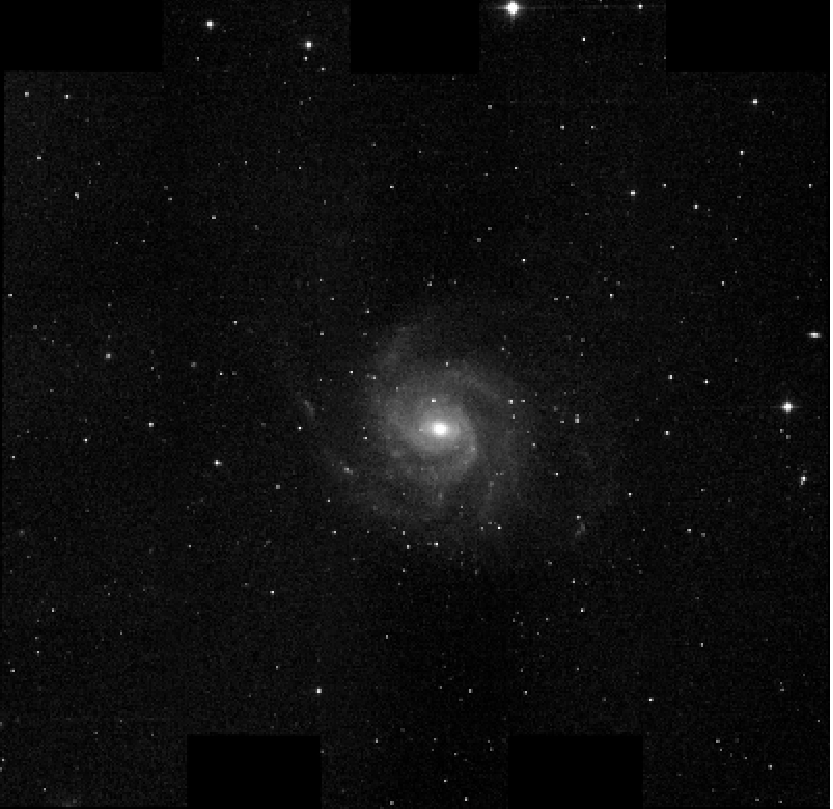
\includegraphics[scale=0.5]{imagens/mosaico2.pdf} 
% 		\caption{Mosaico M101 corrigido.}
% 		\label{fig:MosaicoCorrigido}
% 	    \end{center}
% 	\end{figure}  
    
    \section{Implementação}
    \label{sec:ImplementacaoReal}
	Para implementar e executar o \textit{workflow} Montage foram criados cinco serviços Web, cada um executando uma das etapas do algoritmo mencionadas anteriormente, e um serviço extra responsável por enviar e receber dados da SHARCNET.
	Uma composição BPEL foi desenvolvida conectando os serviços de forma sequencial e configurando a primeira das etapas, a mais custosa, para ser executada na SHARCNET.
	
	A \autoref{fig:ImM101BPEL} demonstra o \textit{workflow} final. Seu código BPEL e resposta final gerada são listados no \autoref{chap:FontesMontage}.
	A SHARCNET é configurada inicialmente com as 10 imagens do Atlas 2MASS da galáxia Pinwheel.
	Em seguida, cada uma das seguintes etapas é executada:
	
	\begin{enumerate}
	 \item O serviço que contém o \textit{workflow} recebe a chamada de inicio e começa a execução.
	 \item Os parâmetros para a chamada ao UDDI estendido são configurados.
	 \item O UDDI estendido é consultado e, nesse caso, deverá retornar o URI para a SHARCNET.	
	 \item Utilizando os parâmetros retornados pelo UDDI estendido, a chamada para a execução na SHARCNET é configurada.
	 \item A primeira etapa do algoritmo Montage é executada na SHARCNET.
	 \item A SHARCNET envia a resposta de forma assíncrona.
	 \item Os parâmetros para o restante do WF são configurados.
	 \item O serviço para executar a transferência de arquivos, obtendo os dados gerados na SHARCNET, é invocado.
	 \item O serviço com a segunda etapa do Montage é invocado.
	 \item O serviço com a terceira etapa do Montage é invocado.
	 \item O serviço com a quarta etapa do Montage é invocado.
	 \item O serviço com a quinta etapa do Montage é invocado.
	 \item Os parâmetros de retorno são preparados.
	 \item Resposta final é retornada.
	\end{enumerate}
	
	\begin{figure}[!htb]%Figura:Imagem BPEL M101
	    \begin{center}
		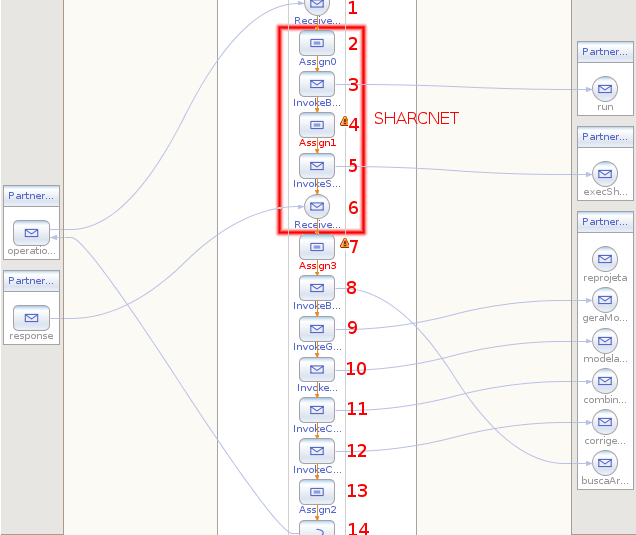
\includegraphics[scale=0.6]{imagens/ImM101BPEL.png}
		\caption{Imagem do BPEL para o \textit{workflow} do Montage.}
		\label{fig:ImM101BPEL}
	    \end{center}
	\end{figure}
	
	Para invocar o BPEL foi utilizado o SOAPUI~\cite{soapui:website}, uma ferramenta de código aberto para a execução de testes em serviços Web. Os Códigos~\ref{cod:logMontage1}, \ref{cod:logMontage2} e \ref{cod:logMontage3}, no \autoref{chap:FontesMontage}, mostram \textit{logs} de execução deste exemplo em horários distintos, com o objetivo de testar a escolha de \textit{clusters} com cargas variadas.

    \section{Discussão}
    \label{sec:DiscussaoReal}
	Alguns fatores importantes devem ser destacados.
	Primeiramente, foi possível resolver o problema através de um \textit{wokflow} escrito em BPEL e executando parte do mesmo na SHARCNET.
	Dessa forma, é possível gerenciar e modificar o processo de uma forma simples, aproveitando as vantagens dos \textit{workflows} e, ao mesmo tempo, utilizar o grande poder computacional de um \textit{Multi-Cluster}.
	Também foi possível notar que utilizar o processamento da SHARCNET foi simples e a alocação de \textit{clusters} foi feita de forma transparente, sempre atendendo aos requisitos do usuário e optando pelos mais disponíveis.
	Entretanto, a movimentação de dados ainda foi feita de forma manual.
	
	Outro fator importante é a dificuldade de se monitorar a execução.
	Como o tipo de \textit{workflow} utilizado possui serviços demorados, que podem levar de minutos a dias em execução, fica difícil saber qual estágio está sendo executado em um determinado momento. Este problema ainda é maximizado quando existem diversas instâncias de \textit{workflow} sendo executadas ao mesmo tempo.
	Neste trabalho o monitoramento foi todo feito baseado nas saídas impressas pelos serviços.
	Entretanto, esse processo poderia ser facilitado com uma ferramenta específica para esse objetivo.
    
    
\chapter{Conclusões}
\label{chap:Conclusao}    

    Esta dissertação descreve uma extensão à linguagem WS-BPEL para atender os requisitos de um \textit{Multi-Cluster}.
    Essa extensão permite a especificação de atributos de QoS e de recursos necessários utilizando WS-Policy.
    Além do mais, este trabalho também propõe uma infraestrutura para a execução de \textit{workflows} em \textit{Multi-Clusters} e sua implementação correspondente na SHARCNET, uma rede multi-institucional de \textit{clusters} de alta performance distribuídos em dezesseis instituições acadêmicas na província de Ontário, no Canadá.
    Em particular, o principal elemento dessa arquitetura é o \textit{Mediador}, que atua como um \textit{proxy} e contém um \texttt{Meta-Escalonador}, que seleciona de forma transparente os \textit{clusters} de acordo com os requisitos dos usuários.

    Diversos trabalhos abordam o problema de especificação e implementação de \textit{workflows} em sistemas distribuídos mas alguns deles implementam novas linguagens para criar a composição, enquanto a tendência é a utilização de padrões já estabelecidos como WS-BPEL.
    Além do mais, não foram encontrados trabalhos que foquem em uma estrutura de \textit{Multi-Cluster}, sendo a maioria deles baseados em grades computacionais.	

    A implementação integra uma máquina de execução WS-BPEL para executar \textit{workflows} na rede SHARCNET através do uso de serviços Web assíncronos e WS-Addressing em conjunto com o UDDI estendido proposto por Garcia e Toledo~\cite{DiegoUDDI}.
    Para cada tarefa de CoC a \texttt{Máquina de Execução} requisita ao \texttt{Escalonador Global} uma seleção de \textit{cluster}.
    Em seguida, a tarefa é submetida e executada no \textit{cluster} escolhido.
    
    A solução se mostrou viável.
    Contudo, trabalhar com BPEL é um processo muitas vezes lento e utilizar funcionalidades que não são comuns é complexo e dependente da máquina de execução que está sendo utilizada.
    Foi possível executar processos utilizando recursos de um CoC, mas como esse tipo de processo pode demorar de minutos a dias em execução, fica difícil saber qual estágio está sendo executado em um determinado momento.

    \section{Contribuições}
	As principais contribuições incluem:
	\begin{itemize}
	 \item Uma extensão à linguagem WS-BPEL para a especificação de \textit{workflows} que podem utilizar recursos de um ambiente Multi-Cluster usando padrões consolidados, como o WS-Policy, permitindo a seleção de serviços baseada em requisitos não-funcionais;
	 \item Uma proposta de arquitetura para a execução de \textit{workflows} em um \textit{Multi-Cluster};
	 \item Um estudo de caso aplicando essa arquitetura na rede SHARCNET;
	 \item Uma implementação de escalonador global para a SHARCNET (Meta-Escalonador);
	 \item Especificação e implementação de um \textit{workflow} científico real, para gerar mosaicos personalizados do céu, utilizando o ambiente criado.	 
	 \item Poster e artigo resumido com o título: ``\textit{A global scheduler for SHARCNET}'' no \textit{SHARCNET Research Day 2009}; Waterloo, Ontário, Canadá \cite{Lechuga2}.
	 \item Artigo completo com o título: ``\textit{An Infrastructure for Executing WS-BPEL Workflows in a Cluster of Clusters}'' no \textit{IEEE symposium on Computers and Communications (ISCC 2010)}; Riccione, Itália\cite{Lechuga1}.
	\end{itemize}

    \section{Trabalhos Futuros}
	Trabalhos futuros incluem o gerenciamento de dados, como armazenamento distribuido e considerações custo para a transferência dos mesmos entre nós;
	Estudos contemplando tolerância a falhas;
	Considerações de reserva, co-alocação e realocação de recursos;
	Consideração de ambientes móveis para a solicitação de serviços;
	E a criação de uma ferramenta para auxiliar no monitoramento do estado de cada \textit{workflow} sendo executado.	

\appendix

  \chapter{Interfaces para a utilização do Mediador}
    %WSDL Mediador
    \section{Interface WSDL para acesso ao Mediador e Callback}
    \lstinputlisting[caption=Interface WSDL para acesso ao \texttt{Mediador}.,language=XML]{listings/WSDL-Mediador.xml}
    \pagebreak
    \section{Interface XSD para acesso ao Mediador e Callback}
    \lstinputlisting[float=!htb, caption=Interface XSD para acesso ao \texttt{Mediador}.,language=XML]{listings/XSD-Mediador.xml}
  
  \chapter{Fontes Completos do Exemplo Montage}   
  \label{chap:FontesMontage}
    %BPEL Montage    
    \lstinputlisting[caption=Código do processo BPEL para a execução do \textit{workflow} Montage.,label=cod:BPEL-Montage, language=XML]{listings/bpel-montage.xml}    
    
    %Politica Montage
    \lstinputlisting[caption=Política de recursos utilizada na aplicação Montage., label=cod:politicaRecursosMontage, language=XML]{listings/policy-rec.xml}

    %Resultado Montage
    \lstinputlisting[caption=Resposta final retornada pelo \textit{workflow} da aplicação Montage., label=cod:respostaMontage, language=XML]{listings/resposta-montage.xml}
    
    %Log execução Montage1
    \lstinputlisting[caption=\textit{Log} de execução da aplicação Montage (1)., label=cod:logMontage1, language=XML]{listings/log-montage1.out}
    
    %Log execução Montage2
    \lstinputlisting[caption=\textit{Log} de execução da aplicação Montage (2)., label=cod:logMontage2, language=XML]{listings/log-montage2.out}
    \pagebreak
    %Log execução Montage3
    \lstinputlisting[caption=\textit{Log} de execução da aplicação Montage (3)., label=cod:logMontage3, language=XML]{listings/log-montage3.out}

%       \includepdf[pages=-]{../Artigos/ISCC2010-OK/artigo.pdf} %includes a five page file

\bibliographystyle{plain}
\bibliography{../Referencial/Cluster-of-Clusters/coc,../Referencial/geral,../Referencial/BPEL-Grid/bpel-grid,../Referencial/WF-GRID/wf-grid,../Referencial/Sharcnet/sharcnet,../Referencial/WS/ws,../Referencial/SOA/soa}

\end{document}
